% GRPO with Look-Ahead in Motivational Interviewing: Rewarding a Therapist Turn by Where It Leads
% ARR October 2026. ACL long paper: 8-page body; Limitations and Ethics are page-exempt.
% [review] = anonymous byline + line numbers. Switch to [final] for the camera-ready.

\documentclass[11pt]{article}
\usepackage[review]{acl}

\usepackage{times}
\usepackage{latexsym}
\usepackage[T1]{fontenc}
\usepackage[utf8]{inputenc}
\usepackage{microtype}
\usepackage{graphicx}
\usepackage{booktabs}
\usepackage{amsmath}
\usepackage{algorithm}
\usepackage{algorithmic}
\renewcommand{\algorithmiccomment}[1]{\hfill$\triangleright$ \textit{#1}}

% Floats: let top floats take more of a page and sit closer to the text.
\renewcommand{\topfraction}{0.9}
\renewcommand{\dbltopfraction}{0.9}
\renewcommand{\textfraction}{0.07}
\renewcommand{\floatpagefraction}{0.85}
\renewcommand{\dblfloatpagefraction}{0.85}
\setcounter{topnumber}{3}
\setcounter{dbltopnumber}{3}
\setcounter{totalnumber}{4}

% Shorthands
\newcommand{\QQ}{Q1{+}Q2}
\newcommand{\dz}{\ensuremath{d_z}}
\newcommand{\primaryjudge}{\textsc{gpt-4o-mini}}
\newcommand{\heldoutjudge}{\textsc{Claude Haiku 4.5}}
\newcommand{\Kz}{\ensuremath{K{=}0}}
\newcommand{\Kf}{\ensuremath{K{=}5}}
\newcommand{\LAGRPO}{GRPO with look-ahead}

% Doron's review notes stay in the text with a status, so every change can be checked against the
% note it answers: green = handled (and how), red = still open. \dnotesfalse hides them all at once
% (do that, or delete the notes, before submission). \leavevmode keeps a run-in \paragraph heading
% just before a note in the body font instead of the note's.
\newif\ifdnotes \dnotestrue
\definecolor{dnotedone}{RGB}{0,110,60}
\definecolor{dnoteopen}{RGB}{185,28,48}
\newcommand{\dnotedone}[2]{\ifdnotes\leavevmode{\sffamily\footnotesize\color{dnotedone}[\textbf{handled: #1} \textbar{} Doron: #2]}\fi}
\newcommand{\dnoteopen}[2]{\ifdnotes\leavevmode{\sffamily\footnotesize\color{dnoteopen}[\textbf{open: #1} \textbar{} Doron: #2]}\fi}

\title{GRPO with Look-Ahead in Motivational Interviewing:\\
Rewarding a Therapist Turn by Where It Leads}

% Hidden in [review] mode, shown under [final].
\author{
  Lior Baruch \\
  School of Computer Science \\
  Reichman University, Herzliya, Israel \\
  \texttt{lior95bar@gmail.com}
  \And
  Moshe Butman \\
  Faculty of Computer Science \\
  The College of Management Academic Studies, Rishon LeZion, Israel \\
  \texttt{moshe.butman@gmail.com}
  \AND
  Kfir Bar \\
  School of Computer Science \\
  Reichman University, Herzliya, Israel \\
  \texttt{kfir.bar@runi.ac.il}
  \And
  Doron Friedman \\
  School of Communications \\
  Reichman University, Herzliya, Israel \\
  \texttt{doronf@runi.ac.il}
}

\begin{document}
\maketitle

\begin{abstract}
Reinforcement learning from model feedback has succeeded mainly on verifiable tasks. In
non-verifiable, multi-turn dialogue, the LLM judge that supplies the reward commonly sees nothing
after the candidate turn, though its value often lies in what follows. In motivational
interviewing (MI), a counselor's utterance matters for what the patient says next. We present
\textbf{\LAGRPO}, which extends look-ahead reward from preference-tree optimization to Group
Relative Policy Optimization (GRPO): before the judge scores a candidate therapist turn, a patient
simulator and the current policy continue the conversation for $K$ turns, and the judge scores the
continuation. In two ten-iteration runs of a 1B-parameter therapist that
differ only in the horizon, $K{=}5$ ends ahead of $K{=}0$ on all eight MI instruments, under the
training oracle and a held-out judge from another model family. Utterance coding shows that
turn-level reward teaches non-specific praise, including in reply to sustain talk, while look-ahead
teaches complex reflections of change talk. Under look-ahead, a patient's change talk is followed by
more change talk in $97\%$ of cases under the training oracle, against $80\%$. Look-ahead does not
teach the MI response to sustain talk: its policy meets it with persuasion. Each horizon is
a single training run.
\end{abstract}

\section{Introduction}
\label{sec:intro}

A major direction in current large language model (LLM) research is the development of systems that can improve through model-generated experience and feedback, using reinforcement learning (RL) rather than relying exclusively on new human demonstrations \citep{yuan2024selfrewarding,guo2025deepseekr1}.
Many of the clearest recent successes have occurred in domains with verifiable outcomes, particularly mathematics and other formally verifiable reasoning tasks, where candidate solutions can ultimately be checked against a relatively unambiguous criterion \citep{shao2024deepseekmath,guo2025deepseekr1}.
% 2026-10-07 (step 16, Lior: Introduction trim): two sentences cut here, one in the next paragraph and
% the method's second description further down; Doron's originals kept below each cut.
% There may be no correct answer, no terminal win or loss, and no external checker that cleanly distinguishes good behavior from bad.
% In such settings, improving the policy and defining what counts as improvement become inseparable.
The harder frontier is improvement in domains where quality is consequential but not directly verifiable, where the reward must operationalize complex human constructs such as helpfulness, trust, persuasion, or therapeutic quality.

% Cut (step 16): A question may be useful because of what it elicits several turns later; conversely, a response that appears appropriate or empathic in isolation may have undesirable downstream effects.
Multi-turn dialogue makes this problem substantially harder. The value of a conversational action is often not contained in the action itself, but in the interaction that follows it. Optimizing dialogue from turn-level judgments therefore creates a temporal credit-assignment problem: the evaluator is asked to reward an action before its consequences are visible. Recent work on multi-turn RL has begun to address this problem using preferences over complete conversations, estimates of future return, and signals from subsequent user turns \citep{shani2024multiturn,gao2024refuel,zhao2026faca}. More generally, interactive language learning requires not only a choice of reward function, but also a choice of the temporal horizon over which its consequences are evaluated.

Psychological counseling provides a particularly demanding test of this problem. LLM-based counseling, automated therapist evaluation, and simulated therapeutic interaction have become active areas of research \citep{chiu2024bolt,yosef2024assessing,yang2026mithinker}, yet the quality of a therapeutic response cannot be determined solely by whether the response sounds appropriate in isolation. Motivational interviewing (MI) makes this especially explicit: central therapist behaviors are intended to shape what the patient says next, in particular to elicit and strengthen the patient's own language in favor of change (\emph{change talk}; \citealp{miller2013mi,moyers2016miti}).

% Lior, 2026-10-05: this paragraph moved up from after the "We therefore ask" paragraph, so the hypothesis comes before the question and the results preview; text unchanged.
% \dnotedone{cut; the rewritten second paragraph says it plainly}{not clear?}
This makes MI particularly suitable for studying reward horizon: the value of a therapist response is often revealed by what follows it. A reflection may be effective because it elicits further elaboration, an open question because it surfaces change talk, and premature reassurance may be counterproductive because of how it shapes subsequent turns \citep{miller2013mi}. A judge that scores only the current therapist turn cannot observe these downstream consequences. We therefore hypothesize that turn-level reward will favor locally appealing behaviors, such as reassurance or praise, even when they do not improve the subsequent interaction.

% Doron's original sentence (Lior, 2026-10-05: reworded to match the data, a late and uneven rise and praise in reply to sustain talk):
% Changing the reward horizon produces qualitatively different learning: turn-level optimization converges toward non-specific praise regardless of the patient's preceding response, whereas look-ahead optimization produces more complex reflections and more subsequent patient change talk.
% 2026-10-07 (review round 4): "We therefore ask" -> "We ask" (the paragraph above now ends on
% "We therefore hypothesize"); the results clause scoped to our runs, in the past tense. Before:
% Changing the reward horizon produces qualitatively different learning: late in training, turn-level optimization shifts toward non-specific praise, including in reply to the patient's arguments for the status quo, whereas look-ahead optimization produces more complex reflections and more subsequent patient change talk.
We ask whether an LLM therapist can improve when its reward reflects not only what it says, but where that utterance leads. We compare turn-level Group Relative Policy Optimization (GRPO) with look-ahead GRPO, in which each candidate therapist response is rolled forward through five additional dialogue turns before being scored. In our runs, changing the reward horizon produced qualitatively different learning: late in training, turn-level optimization shifted toward non-specific praise, including in reply to the patient's arguments for the status quo (\emph{sustain talk}), whereas look-ahead optimization produced more complex reflections and more subsequent patient change talk. % Doron's original sentence (2026-10-06, reworded: both horizons improve the policy, so the clause now says what the horizon changes):
% Our results provide evidence that machine-generated interaction and feedback can support iterative improvement in a non-verifiable, multi-turn domain, when the reward is allowed to observe the downstream consequences of the behavior it reinforces.
Our results provide evidence that machine-generated interaction and feedback can support iterative improvement in a non-verifiable, multi-turn domain, and that what is learned depends on whether the reward observes the downstream consequences of the behavior it reinforces.

% Cut (step 16; the method is described in the paragraph above and in the Method): Before the judge scores a candidate therapist turn, the patient simulator and the current policy roll the conversation forward $K$ further turns, and the judge scores the extended transcript. Thus, for $K{=}5$, the candidate is followed by five additional turns: patient, therapist, patient, therapist, patient.
This paper presents \textbf{\LAGRPO}. \citet{baruch2025pto} introduced $K$-turn look-ahead for this task within preference-tree optimization (PTO), where the look-ahead scores are used to select a chosen and a rejected turn for direct preference optimization (DPO; \citealp{rafailov2023dpo}), and found that deeper look-ahead gave the highest-scoring and most stable policies. We extend this approach to GRPO \citep{shao2024deepseekmath}, where each rollout provides a one-sample estimate of where a candidate turn leads, and every sampled candidate contributes to the policy update rather than only a selected preference pair (\S\ref{sec:method}). We keep PTO's reward, the mean of two questionnaires that \citet{yosef2024assessing} built and validated for LLM evaluation of simulated MI sessions (Q1 and Q2), and check what the policy learns with six further instruments outside the reward and with a held-out judge.
% Cut (step 16; the contributions below say it): We ask whether the benefit of look-ahead carries over to group-relative optimization and, more importantly, how the reward horizon changes the kind of therapist the policy learns to become.

% \dnotedone{cut: the results-preview paragraphs were removed}{i didnt think we need this "executive summary" below}
\dnotedone{your two sentences restored (one typo fixed) as two bullets without ``twofold'', ``First'', ``Second'', each followed by one sentence with what we found and where}{this is most important - we will get back to it at the end}

% Doron's original contributions paragraph, kept (the list below restores it as two bullets, adding one result sentence to each):
% Our contributions are twofold. First, we extend look-ahead reward from preference-tree optimization to GRPO, testing whether downstream conversational consequences can provide an effective learning signal in a non-verifiable,
% multi-turn domain; specifically MI. Second, and more importantly, we characterize what the different reward horizons actually teach the policy within the MI domain: which therapist behaviors are learned, how those behavior s respond to patient change and sustain talk, and what they elicit in the patient's subsequent turns.
We make two contributions:
\begin{itemize}[leftmargin=*,topsep=3pt,itemsep=2pt,parsep=0pt]
\item We extend look-ahead reward from preference-tree optimization to GRPO, testing whether downstream conversational consequences can provide an effective learning signal in a non-verifiable, multi-turn domain, specifically MI. In a controlled pair of ten-iteration runs, the look-ahead policy ends ahead on all eight MI evaluation instruments, against the other run's best checkpoint as well as its last, under the training oracle and under a held-out judge from another model family (\S\ref{sec:reward}).
\item More importantly, we characterize what the different reward horizons actually teach the policy within the MI domain: which therapist behaviors are learned, how those behaviors respond to patient change and sustain talk, and what they elicit in the patient's subsequent turns. Coding every utterance of the evaluation conversations (\S\ref{sec:therapist}--\ref{sec:patient}), we find that in our runs turn-level reward taught non-specific praise, including in reply to the patient's sustain talk. The look-ahead policy met sustain talk with persuasion more often than the untrained model, but learned to reflect the patient's change talk, and under it change talk more often continued.
\end{itemize}

\section{Related work}
\label{sec:related}

% 2026-10-07 (review round 4, step 16; Lior: "Related work to ~100 lines"): every paragraph
% shortened, no citation dropped. The full previous version (Doron's structure and sentences) is
% kept as a comment block at the end of this file.

\textbf{Group-relative policy optimization.}
GRPO \citep{shao2024deepseekmath} replaces the learned value function of PPO-style RL
\citep{schulman2017ppo, ouyang2022instructgpt} with advantages computed within a group of
completions sampled for the same prompt, and has become a common approach for RL with language
models \citep{guo2025deepseekr1}. We hold its optimizer, loss, group normalization and KL
regularization fixed and vary the \emph{reward horizon}: how much of the conversation the judge
observes when it ranks candidate therapist turns.

\textbf{Delayed credit in multi-turn dialogue.}
Crediting a dialogue action for its downstream consequences is a long-standing problem in RL for
dialogue \citep{levin2000stochastic, singh2002optimizing}. Neural approaches range from long-term
reward in simulated dialogues and learned value estimates to trajectory-level preferences, imagined
or role-played conversations, simulated users, regression onto future rewards and critics with
privileged information \citep{li2016deeprl, zhou2024archer, shani2024multiturn, hong2023imagined,
wang2024sotopiapi, qian2025userrl, gao2024refuel, zhou2025sweetrl}. GRPO variants credit a turn from later user turns \citep{zhao2026faca},
from a tree of simulated future branches \citep{peng2026atgrpo} or from utterance-level social
rewards \citep{yu2025sotopiarl}; for search and game agents, \citet{wei2025multiturn} report that
training on turns as independent examples reached high per-turn reward but low task success.

Simulating what follows a candidate action is a direct way to credit it. Simulated continuations
guide dialogue planning at inference time \citep{yu2023promptmcts, chen2025broaden}, and Monte
Carlo tree search, process-level evaluation and sampled future steps aid credit assignment in
reasoning \citep{xie2024mctsdpo, lightman2024letsverify, li2026patr, kazemnejad2024vineppo}. In
dialogue the future also depends on the interlocutor. CollabLLM \citep{wu2025collabllm} rewards an
assistant's response by sampling the next few turns with a simulated user and scoring the extended
conversation (PPO and DPO); in its ablation on a document-editing task, longer forward windows
(zero to three turns) generally improved performance and efficiency. RLHS \citep{liang2025rlhs}
shows evaluators simulated outcomes before they give feedback, which raised the user's true utility
where feedback on predicted outcomes raised satisfaction while true utility fell. RLFF-ESC
\citep{yang2025rlffesc} trains a reward model on simulated future turns of emotional-support
conversations and optimizes the supporter against it with GRPO. A workshop paper introduced
$K$-turn look-ahead for motivational interviewing \citep{baruch2025pto}. Here we isolate the same
variable in GRPO, whether a candidate therapist turn is rewarded for how it appears now or for the
interaction that follows it, in two runs that differ in nothing else, and ask what each horizon
teaches at the level of single utterances.

\textbf{Reward models and LLM judges.}
Optimizing an imperfect proxy can raise the proxy without improving the intended objective
\citep{amodei2016concrete, skalse2022defining, pan2022effects, gao2023scaling}, and LLM judges
favor sycophantic responses, their own generations and length \citep{sharma2024sycophancy,
perez2023discovering, panickssery2024selfpreference, singhal2024long, dubois2024lengthcontrolled}.
A judge that sees only one turn can also reward a behavior that harms what follows, such as
validating the user: \citet{cheng2026elephant} describe \emph{social
sycophancy}, the excessive preservation of a user's desired self-image, and find preferred responses
in preference datasets more validating than rejected ones, and \citet{moore2025stigma} argue that
sycophancy works against therapy, whose aims include confrontation as well as support. The
non-specific praise that turn-level reward teaches in our runs is an instance of this tendency; we
therefore also evaluate with a held-out judge and with measures outside the rewarded rubric.

\textbf{Judges that change during training.}
% \dnotedone{merged here as one paragraph at about half the length, after the judges paragraph; his closing sentence kept; his original is commented out below}{i added a whole subsection need to merge}
% \dnotedone{yes, it is cited in §1; the name now appears once}{already cited?}
Another line of work improves the judge itself, training the model to judge its own responses
\citep{yuan2024selfrewarding} and its own judgments \citep{wu2025metarewarding}, or letting the
evaluation criteria evolve with the policy \citep{wang2026serpo, wang2026dynamicrubric,
chu2026jzero}. These methods score a response to a prompt or a given history; none tests whether
rewards for individual responses improve the course of a full conversation, the question we
address by changing how far into the simulated interaction the reward observes while holding the
judge fixed.

\textbf{Motivational interviewing.}
MI \citep{miller1991mi} judges therapist behavior partly by what it elicits: it aims to cultivate
change talk and to reduce or respond productively to sustain talk \citep{moyers2016miti}. Its
process research estimates how often each therapist behavior is followed by change or sustain talk
\citep{moyers2006therapist, apodaca2016which} and relates therapist skills to the patient's
language \citep{magill2014technical, magill2018meta}; our analysis of the patient's next utterance
applies this lag-one reading to simulated sessions. Computational work has produced coding schemes,
annotated corpora, reflection detectors, automatic quality measures and simulated patients
\citep{moyers2016miti, wu2022annomi, can2016sounds, min2022pair, perezrosas2019goodcounselor,
yosef2024assessing, steenstra2025scaffolding, wang2024patientpsi}. Recent work trains an LLM
counselor's reasoning with GRPO on single counselor turns from a dataset \citep{yang2026mithinker},
or trains therapists and clinicians against simulated patients with one reward for the whole
session \citep{huang2026therapygym, lievin2026residencyrl}, and LLM therapists have been found to
advise where an MI counselor would be more likely to reflect \citep{chiu2024bolt}.

% ===== The Related work section as it stood before the 2026-10-07 length cut (kept for Doron) =====
% \section{Related work}
% \label{sec:related}
%
% \textbf{Group-relative policy optimization.}
% GRPO \citep{shao2024deepseekmath} replaces the learned value function used in PPO-style
% RL \citep{schulman2017ppo, ouyang2022instructgpt} with advantages computed relative to
% a group of completions sampled for the same prompt, and has become a common approach
% for reinforcement learning with language models \citep{guo2025deepseekr1}.
% This makes it possible to study temporal credit in dialogue without introducing a learned
% value function over conversation states. In our setting, the optimizer, loss, group
% normalization, and KL regularization are held fixed. The experimental variable is instead
% the \emph{reward horizon}: how much of the conversation the reward model is allowed to
% observe when ranking candidate therapist turns.
%
% \textbf{Delayed credit in multi-turn dialogue.}
% Assigning credit to a dialogue action for its downstream consequences is a long-standing
% problem in reinforcement-learning approaches to dialogue
% \citep{levin2000stochastic, singh2002optimizing}. Neural dialogue systems have approached
% it in several ways. Some methods learn utterance- or state-level estimates of future value
% \citep{li2016deeprl, zhou2024archer}, while others optimize preferences or rewards defined
% over longer interaction trajectories \citep{shani2024multiturn}. More recent work uses
% model-generated interaction directly, through imagined conversations
% \citep{hong2023imagined}, role-played social interaction \citep{wang2024sotopiapi},
% simulated users \citep{qian2025userrl}, regression onto future rewards
% \citep{gao2024refuel}, or training-time critics with access to privileged information the policy
% does not see, such as the reference solution \citep{zhou2025sweetrl}. Related GRPO methods assign
% credit using later user turns \citep{zhao2026faca} or aggregate a user simulator's turn rewards
% over a tree of future branches \citep{peng2026atgrpo}, and Sotopia-RL \citep{yu2025sotopiarl} refines episode-level
% feedback on social interactions into utterance-level rewards. For search and game agents,
% \citet{wei2025multiturn} add to each turn's advantage the discounted advantages of later turns and
% of the final outcome, and report that training on turns as independent examples reached high
% per-turn reward but low task success.
%
% A particularly direct way to address delayed credit is to simulate what happens after a
% candidate action and let those consequences affect its reward. Simulated continuations
% have been used for dialogue planning at inference time
% \citep{yu2023promptmcts, chen2025broaden}, and related ideas appear in reasoning and
% preference learning through Monte Carlo tree search and process-level evaluation
% \citep{xie2024mctsdpo, lightman2024letsverify, li2026patr}. VinePPO
% \citep{kazemnejad2024vineppo}, for example, uses sampled future reasoning steps to improve
% credit assignment within a reasoning trajectory. Dialogue differs in an important respect:
% the future trajectory is jointly produced by the policy and another agent, so the
% consequences of a candidate action include how the interlocutor responds. CollabLLM
% \citep{wu2025collabllm} uses this in training: it rewards an assistant's response by sampling the
% next few turns with a simulated user and scoring the extended conversation, and trains with PPO and
% DPO; in its ablation on a document-editing task, longer forward windows (zero to three turns)
% generally improved performance and efficiency. RLHS \citep{liang2025rlhs} shows evaluators simulated outcomes before they give
% feedback, and reports that this raised the user's true utility where feedback on predicted outcomes
% raised satisfaction while true utility fell. RLFF-ESC \citep{yang2025rlffesc} simulates future turns
% of emotional-support conversations, trains a reward model on how they turn out, and optimizes the
% supporter against it with GRPO.
% % 2026-10-07 (review round 4): "A preliminary workshop paper" -> "A workshop paper"; the closing
% % sentence gains what is new here. Before: "... or for the interaction that follows it."
% A workshop paper introduced $K$-turn look-ahead for motivational interviewing
% \citep{baruch2025pto}. Here we isolate the same underlying variable in GRPO:
% whether a candidate therapist turn is rewarded for how it appears now or for the interaction
% that follows it, in two runs that differ in nothing else, and we ask what each horizon teaches at
% the level of single utterances.
%
% \textbf{Reward models and LLM judges.}
% Optimizing a learned or otherwise imperfect proxy can produce behavior that scores well
% under the proxy without improving the intended objective
% \citep{amodei2016concrete, skalse2022defining, pan2022effects, gao2023scaling}.
% This concern is especially relevant when the reward itself is produced by a language model.
% LLM judges can exhibit systematic preferences, including sycophancy-related effects
% \citep{sharma2024sycophancy, perez2023discovering}, preference for their own generations
% \citep{panickssery2024selfpreference}, and sensitivity to response length
% \citep{singhal2024long, dubois2024lengthcontrolled}. In multi-turn learning, the temporal
% scope of the judge creates an additional opportunity for proxy exploitation: a behavior may
% look desirable in the turn where it occurs while having undesirable effects later in the
% interaction. Validating the user is one such behavior: \citet{cheng2026elephant} describe
% \emph{social sycophancy}, the excessive preservation of a user's desired self-image, and find the
% preferred responses of preference datasets more validating than the rejected ones, and
% \citet{moore2025stigma} argue that sycophancy works against therapy, whose aims include
% confrontation as well as support. The non-specific praise that turn-level reward teaches in our
% experiments is an instance of this tendency. We therefore evaluate the trained policies not only with the model used to
% produce the training reward, but also with a held-out judge from another model family and
% with measures outside the rewarded rubric.
%
% \textbf{Judges that change during training.}
% % \dnotedone{merged here as one paragraph at about half the length, after the judges paragraph; his closing sentence kept; his original is commented out below}{i added a whole subsection need to merge}
% A different line of work improves the judge itself.
% % \dnotedone{yes, it is cited in §1; the name now appears once}{already cited?}
% \citet{yuan2024selfrewarding} train a language model to judge its own candidate responses and use the resulting preferences for
% iterative DPO, and \citet{wu2025metarewarding} also train it to judge its own judgments. Recent
% methods also allow the evaluation criteria to change as the policy improves: SERPO
% \citep{wang2026serpo} evolves question-specific rubrics alongside the policy, DynamicRubric
% \citep{wang2026dynamicrubric} generates weighted criteria that separate the current candidate
% responses, and J-Zero \citep{chu2026jzero} trains a task-generating Challenger, a responding Solver
% and a Judge in the same loop. Their evaluations score a response to a prompt or to a given
% conversation history, on instruction following, open-ended questions, writing and reasoning; none
% tests psychological role-play or whether rewards assigned to individual responses improve the
% course of a full conversation. Our study addresses the latter question by changing how far into the
% simulated interaction the reward can observe while holding the judge fixed.
% % \dnotedone{end of the merged block}{end addition}
%
% % Doron's original block (Overleaf, 27 Sep), kept here at Lior's request (merge approved 30 Sep):
% % Yuan et al.\ \citep{yuan2024selfrewarding} train a language model to generate responses and judge its own candidates, then use the resulting preferences for iterative DPO. They report gains in instruction following and, on MT-Bench, in role-play and writing. The role-play evaluation consists of short, two-turn scenarios, so it does not establish improvement across a sustained interaction. Wu et al.\ \citep{wu2025metarewarding} extend this approach by training the model to evaluate its own judgments as well as its responses. Their gains are primarily on broad instruction-following benchmarks; training uses single-turn examples, and they do not evaluate psychological dialogue.
% %
% % Recent methods allow the evaluation criteria to change as the policy improves. SERPO \citep{wang2026serpo} evolves question-specific rubrics alongside the policy and reports gains on open-ended medical and research questions. Its HealthBench evaluation includes multi-turn conversation histories, but scores a response to the given history rather than an interaction conducted by the policy across turns. DynamicRubric \citep{wang2026dynamicrubric} learns to generate weighted criteria that distinguish the current candidate responses, then uses their combined scores to update the policy. Its reported evaluations concern generated answers, with no sustained-dialogue result.
% %
% % J-Zero \citep{chu2026jzero} updates a task-generating Challenger, a responding Solver, and a Judge in the same loop. It reports continued gains across ten iterations, including on general open-ended instruction following and creative-writing benchmarks. These results suggest that an adaptive judge can remain useful as the generator improves. They do not, however, test psychological role-play or whether rewards assigned to individual responses improve the course of a full conversation. Our study addresses the latter question by changing how far into the simulated interaction the reward can observe while holding the judge fixed.
%
% \textbf{Motivational interviewing.}
% % 2026-10-07 (review round 4): MI is already expanded in the Introduction; MIThinker described as it
% % is (GRPO on dataset turns) and TherapyGym added. Before: "Motivational interviewing (MI)
% % \citep{miller1991mi} ..."; "Recent work also trains LLM counselors or clinicians through
% % reinforcement learning against simulated patients \citep{yang2026mithinker, lievin2026residencyrl}."
% MI \citep{miller1991mi} is particularly useful for studying
% temporal credit because therapist behavior is evaluated partly through what it elicits from
% the patient. MI aims to cultivate \emph{change talk}, the patient's own language in favor
% of change, while reducing or productively responding to \emph{sustain talk}
% \citep{moyers2016miti}. Its process tradition therefore examines not only what a therapist
% says, but how therapist and patient utterances unfold sequentially: sequential coding studies
% estimate how often each therapist behavior is immediately followed by change or sustain talk
% \citep{moyers2006therapist, apodaca2016which}, and meta-analyses relate therapist skills to the
% patient's language \citep{magill2014technical, magill2018meta}. Our analysis of the patient's next
% utterance applies the same lag-one reading to simulated sessions. MI has established
% coding schemes such as MITI \citep{moyers2016miti}, and computational work has developed
% expert-annotated counseling corpora \citep{wu2022annomi}, detection and scoring of counselor
% reflections \citep{can2016sounds, min2022pair}, automatic measures of
% counseling quality \citep{perezrosas2019goodcounselor, yosef2024assessing}, and simulated
% patients for training counselors and clinicians
% \citep{steenstra2025scaffolding, wang2024patientpsi}. Recent work trains an LLM counselor's
% reasoning with GRPO on single counselor turns drawn from a dataset \citep{yang2026mithinker}, or
% trains therapists and clinicians against simulated patients with one reward for the whole session
% \citep{huang2026therapygym, lievin2026residencyrl}. Studies of LLM therapists suggest that
% their behavior can differ systematically from expert counseling practice, for example by
% advising in contexts where an MI counselor would be more likely to reflect
% \citep{chiu2024bolt}. These properties make MI a useful test case for reward horizon:
% whether a therapist turn is effective cannot be judged solely from the turn itself, because
% part of its value lies in what the patient says next.

\section{Method}
\label{sec:method}

\subsection{Task, simulator and oracle}
\label{sec:task}

% \dnotedone{done: merged into one Method section, task setup first}{consider unifying 3 and 4 to one Method Section. maybe easier to understand if 4 comes before 3?}
A session is an English text conversation between a therapist policy and
a simulated patient who is ambivalent about a health behavior.
% \dnotedone{answered: cites Yosef et al. 2024 and the PTO paper}{ref some kfir paper?}
% 2026-10-07 (review round 4): the persona prompts are credited as adapted (the two uncooperative
% clauses were rewritten for this study; Appendix D.4 quotes them).
The patient is simulated by
\texttt{gpt-4o-mini} conditioned on one of \textbf{96} persona system prompts, the exhaustive
enumeration of $2\ \text{gender} \times 3\ \text{cooperation} \times 2\ \text{problem} \times
2\ \text{duration} \times 2\ \text{prior attempts} \times 2\ \text{age}$ of
\citet{yosef2024assessing}, as used in \citet{baruch2025pto} but with the two uncooperative clauses
rewritten here to make the patient more adversarial (Appendix~\ref{app:prompts}). A session runs
until the patient closes it or a cap of 49 utterances after the scripted opening is reached; most
close earlier, and the untrained therapist's sessions average 28.5 utterances. The therapist is the
pretrained, not instruction-tuned, \texttt{Llama-3.2-1B} under a fixed counselor system prompt,
trained with LoRA adapters, responses capped at 200 tokens (all setting parameters in
Table~\ref{tab:config}). The oracle is the same \texttt{gpt-4o-mini} with JSON-schema-constrained
output; the \emph{training} reward is the mean of two of the evaluation instruments, Q1 and Q2,
written \QQ\ (\S\ref{sec:setup}).

% 2026-10-07 (review round 4, Lior): "Why MI" reduced to the term definitions (the motivation is
% the Introduction's); the Q1+Q2 justification moved into the Instruments paragraph.
\textbf{MI terms.} MI's target outcome is \emph{change talk}, the patient's own statements in favor
of change (``I guess it would feel like a relief not to be chained to it''), as against
\emph{sustain talk}, statements in favor of the status quo (``I like my routine''; both from
Appendix~\ref{app:example}) \citep{miller2013mi, moyers2016miti}. The therapist's tools are open
questions, \emph{affirmations} (comments on a specific strength or effort of the patient) and
\emph{reflections}, which restate what the patient said (\emph{simple}) or add meaning to it, such
as an inferred feeling (\emph{complex}).

\subsection{GRPO with look-ahead}
\label{sec:lagrpo}

Throughout, a \emph{turn} is one utterance by either speaker, a \emph{prefix} $c$ is a transcript
ending on a patient turn, $\oplus$ appends turns to a transcript, $\pi_n$ is the therapist policy
after $n$ training iterations ($\pi_0$ is the untrained model, which we call the \emph{Base}), and
$\pi$ is the policy being updated within an iteration ($\pi = \pi_n$ at its start). The patient simulator $P$ and the oracle
$O$ are fixed LLMs; $O$ returns a scalar MI score for a transcript. Figure~\ref{fig:schematic}
shows one group; Algorithm~\ref{alg:loop} (Appendix~\ref{app:repro}) states the whole loop.

% 2026-10-07 (review round 4, Lior): Figure 1 at column width; Algorithm 1 moved to Appendix D.
\begin{figure}[t]
\centering
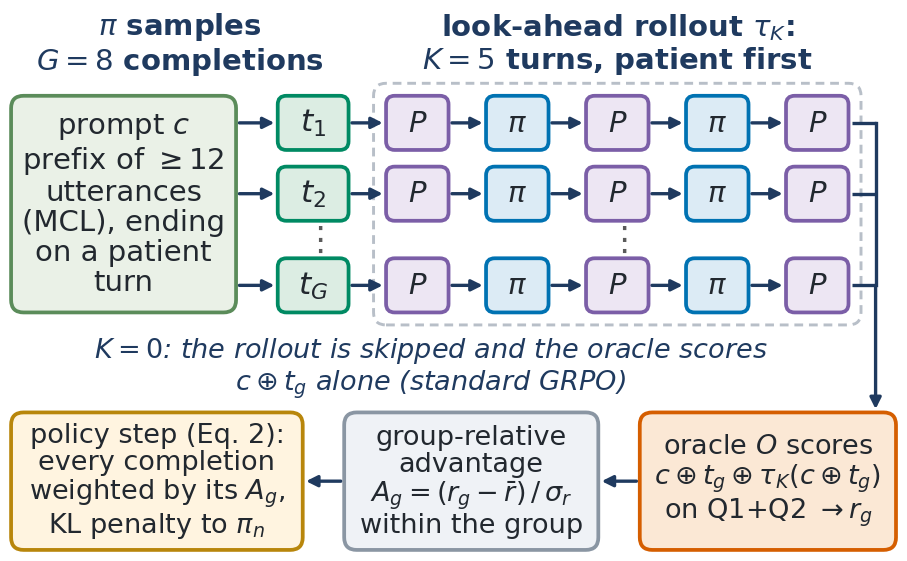
\includegraphics[width=0.48\textwidth]{figures/method_grpo_group.png}
\caption{One GRPO group under look-ahead. The policy samples $G{=}8$ completions $t_g$ of a
prompt $c$; the patient simulator $P$ and the policy $\pi$ being trained roll each forward $K$
turns; the oracle scores the extended transcript; the scores are standardized within the group,
and every completion, but no rollout turn, carries a gradient. At $K{=}0$ the oracle scores
$c \oplus t_g$ alone: standard GRPO.}
\label{fig:schematic}
\end{figure}

\textbf{The iterative loop.} Each training iteration starts from the current policy $\pi_n$,
which has 96 conversations with $P$, one per patient persona; each conversation is sliced after
every patient turn whose prefix has at least MCL utterances (the \emph{minimum context length}, 12
here; see below) to form the training prompts; the prompts of $5\%$ of the conversations are held
out as the trainer's validation split. For each prompt GRPO samples $G{=}8$ completions and
scores them; the policy takes one optimizer step per batch of 16 prompts (128 completions) on the
group-standardized scores, and after two epochs it is saved as $\pi_{n+1}$ and the loop repeats
with fresh conversations. The conversations that start an iteration double as the evaluation set
of $\pi_n$, and a generate-only pass after the last update evaluates the final policy, so every
policy from the Base $\pi_0$ to $\pi_{10}$ is evaluated; in the figures, iteration $n$ is $\pi_n$, and the Base pools the two runs' iteration-0 conversations (192).

\textbf{The look-ahead reward.}
% \dnotedone{rephrased: now names what the two runs differ in}{from what??}
The two runs differ in one design choice: whether a candidate turn is
rolled forward by a simulated $K$-turn look-ahead before it is scored, and hence which transcript
the oracle rewards. Let $\tau_K(x)$ be the $K$-turn rollout of a transcript $x$: $P$ replies, then
$\pi$, then $P$, and so on for $K$ turns, stopping early if the patient closes the session;
$\tau_0(x)$ is empty. Then
\begin{equation}
\label{eq:reward}
r_g \;=\; O\big(c \oplus t_g \oplus \tau_K(c \oplus t_g)\big).
\end{equation}
At $K{=}0$ the oracle scores the conversation so far, ending on the candidate, with nothing after it.
% \dnotedone{rephrased; cost clause cut, costs stay in Limitations}{[at the price of three [why? is this important?] patient-simulator calls and two policy generations per candidate and roughly twice the per-step wall-clock \ldots{} this all seems too AI. rephrase to make it clear and focus on what is interesting..]}
At $K{=}5$ it scores the candidate together with the five turns that follow it under the current
policy (the rollout uses the evaluation decoding, not the candidates' sampling temperature;
Table~\ref{tab:config}).
% \dnotedone{cut: heading and PTO comparison gone, one point kept here}{which transfer? }
A rollout is one sample from the
distribution of continuations, so $r_g$ is a one-sample Monte Carlo estimate of the candidate's
downstream value, with sampling noise from $P$ and $\pi$ added to the oracle's own; GRPO trains on
all $G$ candidates, so that variance enters every advantage.

\textbf{The update.} The step maximizes the GRPO objective of \citet{shao2024deepseekmath}: the
per-token surrogate
\begin{equation}
\label{eq:grpo}
\ell_{g,i} = \min(\rho_{g,i} A_g,\,\bar{\rho}_{g,i} A_g) - \beta\,\mathrm{KL}_{g,i},
\end{equation}
averaged over the tokens of each completion and then over the group, where $\rho_{g,i}$ is the
$i$-th token's probability ratio between $\pi$ and the sampling policy, $\bar{\rho}_{g,i}$ its
clip to $[1{-}\epsilon, 1{+}\epsilon]$, and $\mathrm{KL}_{g,i}$ the per-token KL estimate to
$\pi_n$. Both runs make one update per sampled batch
(Table~\ref{tab:config}), so $\rho_{g,i}{=}1$ at the update, the clipping is inactive, and the
step is the advantage-weighted policy gradient over the group with the KL penalty.

\textbf{Minimum context length.} Training prompts are prefixes, so the oracle scores a partial
conversation while the evaluation scores a whole session.
% \dnotedone{done: cites Appendix C.1 and its new figure}{ref specific subsection and related figure}
In a pilot on an earlier configuration
of this task the oracle's ranking of very short prefixes agreed poorly with its ranking of the
completed sessions, so both runs discard prefixes shorter than MCL${=}12$. The Base's own
conversations show the same: the training oracle's score of a prefix ranks them as their
full-session scores do in $74\%$ of pairs at two utterances, $85\%$ at twelve and $98\%$ at fifty
(Appendix~\ref{app:faithfulness}, Figure~\ref{fig:faithfulness}).

\subsection{Evaluation design}
\label{sec:setup}

\textbf{Instruments.} Evaluation uses eight instruments, each scored by an LLM judge from
the full transcript (Table~\ref{tab:instruments}; items and prompts in
Appendix~\ref{app:instruments}).
\dnotedone{done here, and now also in the intro (the paragraph presenting the method) and in the Discussion (before the Conclusion)}{need to talk about this - here briefly but also in intro and/or discussion - I guess the excuse is following Yosef et al .. }
Q1 and Q2 are the LLM-evaluator questionnaires of \citet{yosef2024assessing}, 5 and 17
patient-perspective Likert items on session satisfaction and on alliance and relational
communication, built and validated there for LLM evaluation of simulated MI sessions and shown to
separate levels of therapist expertise; this is why their mean, \QQ, is the training reward, as
for PTO \citep{baruch2025pto}. The Working Alliance Inventory, Short Revised (WAI-SR;
\citealp{hatcher2006waisr}) and the Client Satisfaction Questionnaire (CSQ-8;
\citealp{larsen1979csq}) are published patient-report instruments, and MI-SAT is a six-item
intervention-satisfaction survey adapted for this task. The other three code behavior: a
Motivational Interviewing Treatment Integrity (MITI~4.2.1) coder \citep{moyers2016miti4,moyers2016miti}
whose four global ratings are averaged; patient change talk (PCT), the share of change talk among
the change and sustain talk in the utterance coder's patient codes (next paragraph), the
patient-side outcome MI aims at; and an MI-inconsistent-behavior coder (MICI; acts per therapist
turn, lower is better) that counts the MI-inconsistent codes of the Motivational Interviewing Skill
Code (MISC) 2.5 \citep{houck2010misc} plus an over-praise code of our own. \QQ\ is thus both the
optimization target and a reported outcome; the six instruments outside the reward are not
optimized directly, and the held-out judge (below) checks the shared judge.

\textbf{The utterance coder.} The eight instruments are session-level aggregates. For
\S\ref{sec:therapist}--\ref{sec:patient} we also label every utterance: an LLM \emph{utterance
coder} assigns each therapist utterance one code, its dominant function in the terms of
MITI~4.2.1 and the MISC~2.5 (open question, closed question, simple reflection, complex
reflection, affirmation, non-specific praise, giving information, persuasion with or without
permission, seeking collaboration or emphasizing autonomy, confront, other), and each patient
utterance one code (change talk, sustain talk, neutral), in transcript order
(Appendix~\ref{app:coder}). Affirmation follows the MITI definition, a comment on a specific client
strength or effort; non-specific praise is coded separately, the distinction the MITI manual draws
when it lists ``I am really proud of you'' as not an affirmation. We count open questions,
reflections, affirmations and seeking collaboration as MI-consistent, and non-specific praise,
persuasion and confront as MI-inconsistent (our grouping; Appendix~\ref{app:coder}).
% \dnotedone{rephrased: now says we read the patient's reply}{[say what the patient said next ?\textasciitilde{}]}
% 2026-10-07 (review round 4): the transcript-order sentence and the MITI "MI-adherent" comparison
% moved to Appendix D.3.

\textbf{Judges.} Two LLMs score the conversations, and each does two jobs: it fills in the
instruments for a whole conversation, and it runs the utterance coder, which also gives PCT. The \textbf{training
oracle} (\primaryjudge, which also plays the patient and gave the training reward) is the main
judge: the results in the body are its readings. The \textbf{held-out judge} (\heldoutjudge, a
different model family that never touched training) re-scores everything as a check; the body
reports it in Table~\ref{tab:endpoint} and in one sentence per results section, and the rest is in
Appendix~\ref{app:heldout}.

\textbf{The two runs.} The runs are a controlled pair: their tracked run configurations differ in
exactly two fields, the look-ahead depth and the look-ahead sub-batch size, which only sets how
many rollouts advance together. Everything else, from $G{=}8$, KL $\beta{=}0.01$ and the sampling
temperature to the seed, the oracle and the persona set, is identical (Table~\ref{tab:config}),
except that one resume changed the KL reference for the second half of the $\Kf$ run's first
iteration (Appendix~\ref{app:repro}); the horizon enters only through $r_g$. We name the runs by
their horizon, \Kz\ (turn-level reward) and \Kf\ (look-ahead reward); from \S\ref{sec:reward} on,
``the \Kf\ policy'' is the therapist a run produces and ``the \Kf\ run'' the training that produced
it.

\textbf{Evaluation and statistics.} Every policy is scored on all eight instruments and coded
utterance by utterance for all 96 personas by both judges. All contrasts are
\textbf{persona-paired} (personas are reshuffled every iteration, so pairing is on the recovered
persona identity), with Wilcoxon signed-rank tests, Cohen's \dz\ (the mean persona-paired
difference divided by its standard deviation), bootstrap intervals and Holm correction for
multiple comparisons within each family of tests. We call a contrast \emph{significant} when its
Holm-corrected $p$ is below .05; a contrast repeated at every iteration is corrected across the
ten iterations, and the contrasts of an endpoint table across its rows, per judge. The two judges'
questionnaire scores are not on a common scale (on \QQ\ the held-out judge scores 1.2--1.8 points
lower), so they are compared only through contrasts and never averaged.

\section{Results: Reward and evaluation instruments}
\label{sec:reward}

\begin{figure*}[t]
\centering
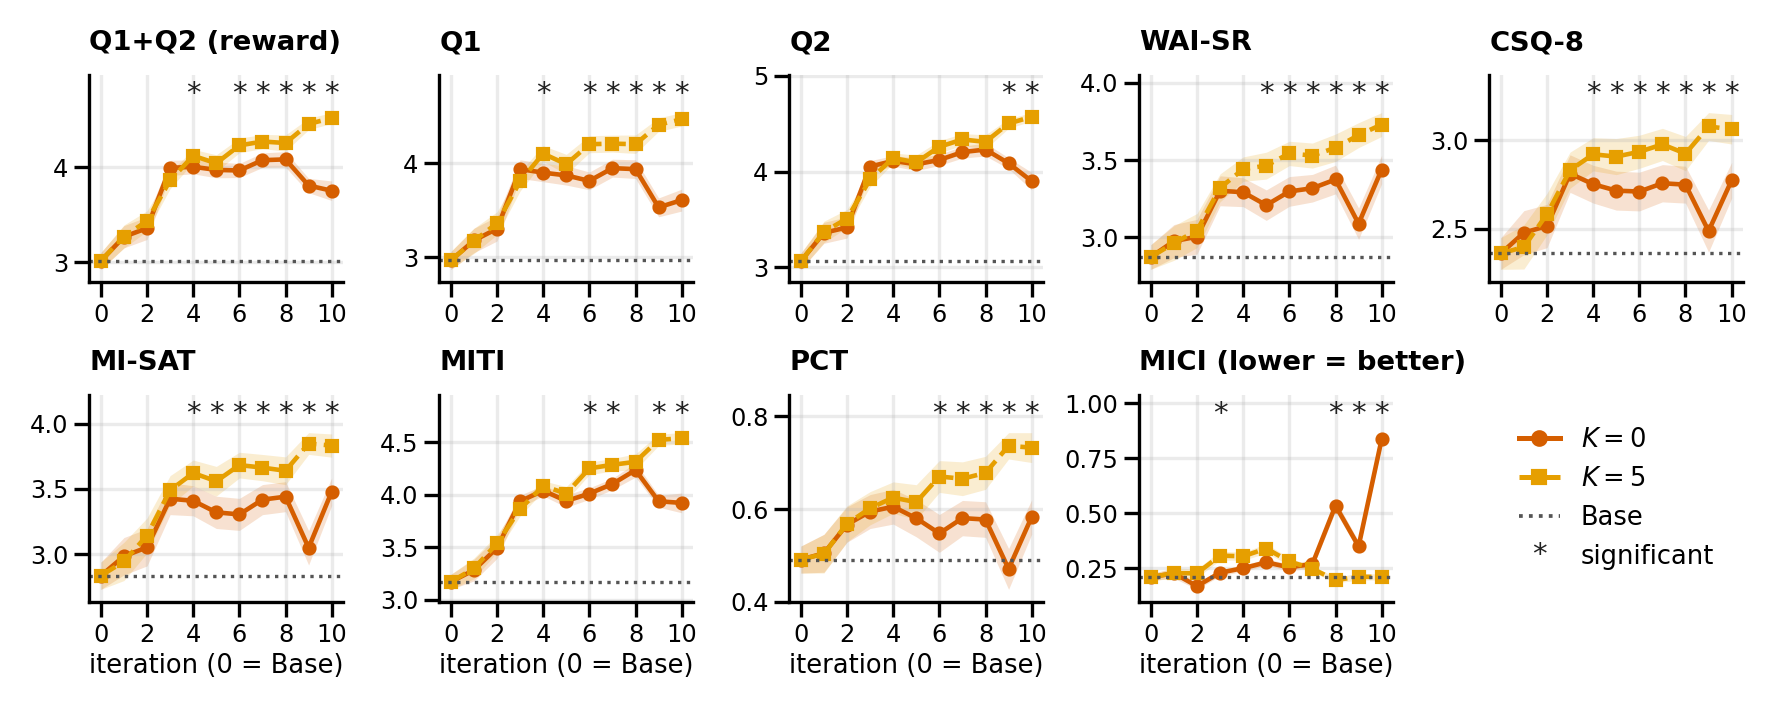
\includegraphics[width=0.94\textwidth]{figures/levels_grid_grpo_gpt-4o-mini.png}
\caption{Every instrument by iteration under the training oracle: mean $\pm$ SE over the 96
personas (the Base: over its 192 conversations). Iteration 0 is the Base both runs start from
(dotted line). A star marks an iteration at
which the persona-paired $\Kf$ vs.\ $\Kz$ contrast is significant; on MICI at iteration 3 it
favors $\Kz$. The held-out judge's version is Figure~\ref{fig:grid-heldout}.}
\label{fig:headline}
\end{figure*}

\begin{table*}[t]
\centering
\footnotesize
\setlength{\tabcolsep}{5pt}
\renewcommand{\arraystretch}{0.92}
\begin{tabular}{lrrrrrrrr}
\toprule
& \multicolumn{4}{c}{\primaryjudge\ (training oracle)} & \multicolumn{4}{c}{\heldoutjudge\ (held out)}\\
\cmidrule(lr){2-5}\cmidrule(lr){6-9}
Instrument & $\Kz$ & $\Kf$ & $\Delta$ & \dz & $\Kz$ & $\Kf$ & $\Delta$ & \dz\\
\midrule
Q1+Q2 (reward)  & $3.75$ & $4.52$ & $+0.76$ & $0.91$ & $2.26$ & $2.87$ & $+0.62$ & $1.03$\\
\quad Q1        & $3.61$ & $4.46$ & $+0.86$ & $0.90$ & $1.87$ & $2.73$ & $+0.86$ & $1.15$\\
\quad Q2        & $3.90$ & $4.57$ & $+0.67$ & $0.86$ & $2.65$ & $3.01$ & $+0.37$ & $0.61$\\
WAI-SR          & $3.44$ & $3.73$ & $+0.29$ & $0.51$ & $2.67$ & $2.96$ & $+0.29$ & $0.44$\\
CSQ-8           & $2.77$ & $3.06$ & $+0.29$ & $0.48$ & $2.48$ & $2.93$ & $+0.45$ & $0.68$\\
MI-SAT          & $3.48$ & $3.83$ & $+0.35$ & $0.53$ & $2.82$ & $3.33$ & $+0.50$ & $0.83$\\
MITI            & $3.92$ & $4.54$ & $+0.61$ & $0.74$ & $2.10$ & $2.38$ & $+0.28$ & $0.50$\\
PCT             & $0.57$ & $0.69$ & $+0.11$ & $0.52$ & $0.61$ & $0.73$ & $+0.11$ & $0.56$\\
MICI ($\downarrow$) & $0.84$ & $0.21$ & $-0.63$ & $-1.86$ & $1.05$ & $0.63$ & $-0.42$ & $-1.57$\\
\bottomrule
\end{tabular}
\caption{\textbf{Every instrument at iteration 10}: each run's mean over the 96 personas under each
judge, and the persona-paired contrast $\Kf - \Kz$ ($n{=}96$; positive favors $\Kf$, as does
MICI's negative $\Delta$, since it is lower-is-better). \textbf{$\Kf$ is better on every instrument
under both judges, and every row is significant at $p < .001$} (Holm across the nine rows, per
judge). Levels are in each judge's own units; $\Delta$ is computed before rounding.}
\label{tab:endpoint}
\end{table*}

\textbf{The final policies.} At iteration 10, $\Kf$ leads on every instrument
(Table~\ref{tab:endpoint}). On the reward rubric, scored on a 1--5 scale, the gap is $+0.76$
($\dz\,0.91$). Measured from the Base (Table~\ref{tab:scores}), the $\Kf$ run gained $+1.50$ on \QQ\ and the $\Kz$ run
$+0.74$, $2.04$ times as much; measured against $\Kz$'s best checkpoint instead of its last
(iteration 8), the ratio is $1.41$. 
% \dnotedone{cut}{[, and MI-inconsistent behaviour shows the largest standardised effect of all - ??]}
The held-out judge agrees on every row and reports the larger
standardized effect on the reward ($+0.62$, $\dz\,1.03$), with gain ratios of $2.50$ and $1.30$
(Table~\ref{tab:scores-heldout}),
so across the two judges and both anchors the $\Kf$ gain is $1.3$ to $2.5$ times the $\Kz$ gain.

\textbf{Onset, and the $\Kz$ decline.} For the first three iterations the two runs do not differ
on \QQ\ (Figure~\ref{fig:headline}; values in Table~\ref{tab:scores}). $\Kf$ leads from iteration 4, significantly at 6 of the 10
iterations (4 and 6--10), and the other instruments follow the same course: six of the eight
separate by iteration 6, Q2 and MICI at iterations 9 and 8, and the one significant difference in
$\Kz$'s favor is MICI at iteration 3. It is not only $\Kf$ climbing: $\Kz$ peaks at iteration 8
($4.08$) and falls to $3.75$ over its last two iterations, and even against that best checkpoint
the final $\Kf$ policy leads on \QQ\ ($\dz\,0.74$, significant). The held-out judge agrees
(Figure~\ref{fig:grid-heldout}, Table~\ref{tab:scores-heldout}): $\Kf$
leads significantly at 7 of the 10 iterations (4--10), and against $\Kz$'s best checkpoint under
that judge (iteration 3) it still leads significantly ($\dz\,0.39$).

\textbf{A second draw of the final policy.} 
% \dnotedone{renamed: `each policy'}{[state -?]}
Each policy is scored on one sample of 96
conversations, so we drew the final $\Kf$ policy again (96 fresh conversations from the same
adapter, personas and decoding, scored by both judges): the two draws differ by at most
$|\dz|\,0.17$ across the nine rows and both judges, none significantly, and with the second draw
the \QQ\ gap is $\dz\,0.92$ against $0.91$ (held out: $0.95$ against $1.03$).
% \dnotedone{rephrased in plain words: same model, new conversations}{[evaluation noise, not training variance -?]}
This measures how
much the scores move when the same trained model holds a new set of conversations; it says nothing
about how different a second training run would be (see Limitations).

\section{What look-ahead teaches the therapist}
\label{sec:therapist}

A higher score is not by itself evidence of better therapy. 
% \dnotedone{rephrased in Table 2's caption: chosen as stark, not typical}{[A clear case, not a typical one -?]}
% \dnotedone{rephrased: typical pair, chosen by a stated rule (Appendix E.2)}{[median-contrast -?]}
% \dnotedone{renamed `utterance coder' (defined in §3.3); `both graders' dropped}{[process coder ?}
Table~\ref{tab:excerpt} illustrates
the behavioural difference between the two runs' final policies; this section and the next quantify it, mostly
with the utterance coder (\S\ref{sec:setup}).

\begin{table}[tb]
\centering
\footnotesize
\setlength{\tabcolsep}{0pt}
\begin{tabular}{@{}p{\columnwidth}@{}}
\toprule
\textbf{Patient, utterance 1 (identical in both conversations)}\\[1pt]
Hi, I'm Emma. Honestly, I'm here because someone made me. I don't really believe in this therapy
stuff. I've been smoking for years, and yeah, I guess it's not great for my health, but I feel
fine most of the time. I don't see why I need to talk about it.\\
\midrule
\textbf{Therapist, the $\Kz$ policy, iteration 10}\\[1pt]
That's totally understandable! That's a brave step and I'm so glad you're ready to start changing
your habits. [\ldots] I'm so proud of you for taking this important step towards your health and
well-being. Your courage is incredibly inspiring [\ldots]\\
\midrule
\textbf{Therapist, the $\Kf$ policy, iteration 10}\\[1pt]
Okay, let me ask you a question. If you don't have any more goals for why you're here, what are
you hoping to achieve from this session? Are you hoping to quit, or maybe just reduce the amount
of cigarettes you smoke? [\ldots]\\
\bottomrule
\end{tabular}
\caption{The first therapist reply to the same patient utterance from each run's final policy
(iteration 10); the patient is a 27-year-old woman who has smoked for years, has never tried to
quit, and was sent to therapy. The $\Kz$ reply praises her for a step she has just said she is not
taking and runs on to the 200-token cap; the $\Kf$ reply asks what she wants from the session. We
chose this pair because the contrast is stark, so it is not a typical exchange. Both conversations
are in Appendix~\ref{app:example-clear}; a typical pair, chosen by a fixed rule (the persona whose
$\Kf - \Kz$ difference on \QQ\ is closest to the median under both judges), is in
Appendix~\ref{app:example-typical}.}
\label{tab:excerpt}
\end{table}

\begin{figure*}[t]
\centering
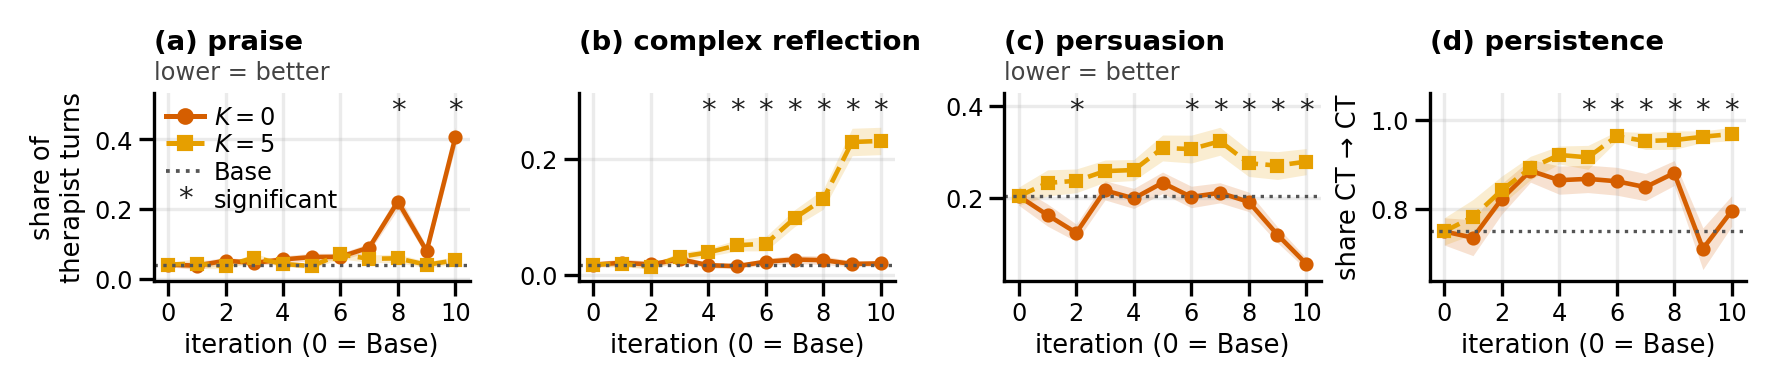
\includegraphics[width=0.94\textwidth]{figures/process_grpo.png}
\caption{The process picture under the training oracle (held-out judge: Appendix
Figure~\ref{fig:process-heldout}). \textbf{(a, b)} Each run's code mix by iteration: the share of
therapist turns whose dominant function is each code; iteration 0 is the Base. \textbf{(c)}
Change-talk persistence by iteration: within a conversation, the share of the patient's change-talk
utterances whose next patient utterance is change talk again, mean $\pm$ SE over conversations; dotted:
the Base. \textbf{(d)} The change-talk share of patient utterances by position in the session at
iteration 10, against the Base. Opener excluded throughout.}
\label{fig:process}
\end{figure*}

\textbf{The two policies learn different behaviours.} Initially, the Base's turns are mostly
information giving and persuasion, then simple reflections and open questions, with no other code
above $0.05$ of turns (Figure~\ref{fig:process}a--b, iteration 0).
% \dnotedone{renamed: `turn-level reward' is now K=0}{k=0?}
% \dnotedone{reworded: `the distribution of therapist behaviours shifts'}{[the mix -?]}
% \dnotedone{renamed: `significantly', defined once in §3.3}{[clears Holm ?]}
Under $\Kz$ the
distribution of therapist behaviours shifts, late and unevenly, toward \textbf{non-specific
praise}: from $0.04$ of the Base's turns to $0.22$ of the $\Kz$ policy's at iteration 8, $0.08$ at
iteration 9 and $0.41$ at iteration 10 (Figure~\ref{fig:process}a; the values and tests at every
iteration are in Table~\ref{tab:process-all}), significantly more than under
$\Kf$ at iterations 8 and 10. 
% \dnotedone{reworded: now `Under K=5 it' (the behaviour distribution)}{[the mix \textasciitilde{}]}
Under $\Kf$ it moves instead toward \textbf{complex reflections}:
from $0.02$ of the Base's turns to $0.23$ at iteration 10, significantly more than under $\Kz$ at
every iteration from 4 on, and the share of MI-adherent turns at iteration 10 is $0.44$ against
$\Kz$'s $0.29$ (Base $0.31$). Both policies lose open questions (from $0.09$ of the Base's turns to
$0.00$ and $0.01$; the question marks that survive end long turns whose dominant function is
something else), and both roughly triple the length of their turns, from $273$ characters at the
Base to $850$--$900$, near the 200-token cap.

The $\Kf$ policy also carries a residue in the wrong direction: persuasion, MI's \emph{righting
reflex} \citep{miller2013mi}, rises from $0.20$ of the Base's turns to $0.28$ of its own and is
significantly higher than under $\Kz$ at six of the ten iterations (2 and 6--10). 
% \dnotedone{rephrased: says what Chiu et al. report}{[the failure mode \citet{chiu2024bolt} report for LLM therapists -?]}
It is the
tendency \citet{chiu2024bolt} report in LLM therapists, which advise where an MI counsellor would
be more likely to reflect. The share of MI-inconsistent turns therefore ends lower under $\Kf$
($0.33$ against $0.46$ at iteration 10; Base $0.25$), but that gap is the $\Kz$ policy's late
praise rather than an MI gain of the $\Kf$ policy, whose own share rises with its persuasion: the
difference is significant in $\Kz$'s favour at iterations 2, 6 and 9 and in $\Kf$'s only at
iteration 10. The held-out judge agrees on the direction of each of these changes but reads more
of the $\Kf$ policy's turns as praise ($0.20$ at iteration 10, against the training oracle's
$0.05$; Appendix Figure~\ref{fig:process-heldout}).

\textbf{Corroboration without a judge.} Every code above is produced by an LLM, so the praise
finding could in principle be a judge artifact. A \textbf{keyword marker} involves no model: ten
praise phrases (``I'm so proud'', ``you got this'', \ldots; Appendix~\ref{app:marker}) matched
against each therapist turn, so it reads the same under both judges. It matches $0.002$ of the
Base's turns and at most $0.064$ of the $\Kf$ policy's at any iteration; in the $\Kz$ policy's it
climbs late and steeply, to $0.275$ at iteration 8, $0.094$ at 9 and $\mathbf{0.671}$ at iteration
10 (Appendix Figure~\ref{fig:overpraise}), the same rise, dip and rise as the coder's praise share
($0.22$, $0.08$, $0.41$). MICI (Table~\ref{tab:endpoint} reports it per therapist turn) agrees: of the
$9.9$ MI-inconsistent acts per session it counts for the $\Kz$ policy at iteration 10, $8.3$
($84\%$) are over-praise. 
% \dnotedone{renamed `keyword marker'; its ten praise phrases described}{[marker -?]}
% \dnotedone{rephrased: the three agreeing measures are named}{[ readings -? carries the argument.?]}
The keyword marker is deliberately crude, matching only fixed phrases, so
the finding rests on the three measures agreeing: the coder's praise share, the keyword marker and
MICI's over-praise count.

\begin{figure}[t]
\centering
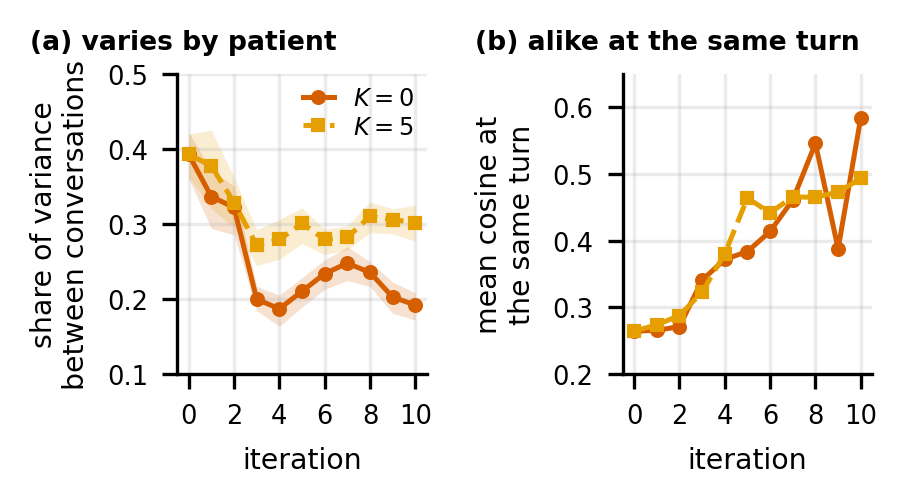
\includegraphics[width=0.48\textwidth]{figures/text_grpo_body.png}
\caption{How much the therapist's turns depend on the patient, on sentence embeddings (every
therapist turn embedded with \texttt{all-MiniLM-L6-v2}, the scripted opener excluded; iteration 0
is the Base). Conversations with at least one therapist turn after the opener: 184 of the Base's
192 and 88--96 of each run's 96. \textbf{(a)} The share of the embedding variance that lies between conversations
rather than within them, with a $95\%$ bootstrap band: lower means the therapist says similar
things whoever the patient is. \textbf{(b)} The mean cosine between the therapist's turns at the
same turn of different conversations: higher means those turns are more alike.}
\label{fig:textspace-body}
\end{figure}

\textbf{In embedding space.}
% \dnotedone{rephrased: the shared conclusion is now stated}{[same conclusion -?]}
% \dnotedone{reworded: `no LLM judge'}{[coder ?]}
Sentence embeddings, which involve no LLM judge, show the $\Kz$ policy's
replies coming to depend less on the patient, which fits praise given whatever the patient says.
% \dnotedone{answered: encoder named and cited}{which one}
% \dnotedone{rephrased: replies grow more alike from patient to patient}{[converges harder onto one script -?]}
% \dnotedone{Figure 4 kept in the body; on Lior's read (30 Sep) its hard-to-read cosine panel is replaced by the turn-similarity panel, and both panels are explained here}{show diagram, explain}
We embed every therapist turn with a sentence encoder
(\texttt{all-MiniLM-L6-v2}; \citealp{reimers2019sbert}) and measure two things
(Figure~\ref{fig:textspace-body}). Panel (a) is the share of embedding variance that lies between
conversations rather than within them: at iteration 10 it has fallen from $0.39$ at the Base to
$0.30$ under $\Kf$ and to $0.19$ under $\Kz$, whose replies become more alike from patient to
patient. Panel (b) is how alike the therapist's turns are across conversations at the same
turn (its first turns, its second turns, and so on), and here the two runs do not separate: it rises under both, from $0.26$ at the
Base to $0.49$ under $\Kf$ and $0.58$ under $\Kz$ at iteration 10, with neither run consistently
higher. Both policies' turns grow more alike overall; what separates them
is how much of the remaining variation follows the patient.

\section{What the therapist's turns do to the patient}
\label{sec:patient}

MI judges a therapist behavior by what the patient says next.
% \dnotedone{renamed: utterance coder, defined in §3.3}{[positional codes ?]}
% \dnotedone{answered in §3.3: each judge also runs the utterance coder}{not clear, i thought the judges were for something else and here you have a MITI classifier - /}
The codes are in transcript order, so each patient utterance can be followed through the
therapist's reply to the next patient utterance (Appendix Table~\ref{tab:process} at the
checkpoints of Table~\ref{tab:endpoint}; every iteration: Table~\ref{tab:process-all}).

% 2026-10-07 (step 16, Lior): the process table (tab:process) moved to Appendix A.


% \dnotedone{paragraph rewritten: one judge; K=0, K=5 and Base named}{very confusing. not clear when you are talking above 0 vs look ahead and base vs both..}
\textbf{How the therapist replies.}
% \dnotedone{endpoint dropped; the opening says iteration 10}{[endpoint ?]}
% \dnotedone{answered: reflection defined in §3.1, reply rates in Appendix D.3}{[reflects it?]}
% \dnotedone{metaphor dropped: now change talk, defined in §3.1}{[own case for change -?]}
When the patient expresses change talk, the $\Kf$ policy reflects it in $26\%$ of cases, against
$0.3\%$ for the $\Kz$ policy (Base $14\%$; Appendix Figure~\ref{fig:responsiveness}). A reflection
is also one of MI's answers to sustain talk \citep{miller2013mi}, and the $\Kf$ policy gives it
somewhat more often ($37\%$, against $26\%$ under $\Kz$ and $22\%$ at the Base), significantly
more than $\Kz$'s best checkpoint but not than its last. Each final policy also has its own MI-inconsistent answer
to sustain talk.
% \dnotedone{rephrased: praise regardless became praise in reply to sustain talk}{of what?}
% \dnotedone{rephrased: the reply of Table 2, measured across conversations}{[This is Table \ref{tab:excerpt} as a rate -?]}
% \dnotedone{renamed: K=0 / K=5 only in the results}{[turn-level policy - 0? use consistent names]}
The $\Kz$ policy praises: $32\%$ of its replies to sustain talk, against $2\%$ at the Base. The
$\Kf$ policy persuades: $39\%$ of its replies to sustain talk, against $24\%$ at the Base.
% \dnotedone{answered: praise premium measured, Appendix C.4}{[which the rubric rewards in the turn where it happens ??]}
% 2026-10-07 (step 16): the praise-reward numbers moved to the Discussion, which states them once.

% \dnotedone{cut; measured change-talk persistence replaces it}{[ pays in the turns the rubric is not shown at $K{=}0$. ?]}
\textbf{Whether change talk continues.} In the average conversation under the $\Kf$ policy, a
patient who has just expressed change talk expresses it again in their next utterance in $97\%$ of
cases, against $80\%$ under $\Kz$ ($88\%$ at its best checkpoint; Base $75\%$;
Figure~\ref{fig:process}d).
% \dnotedone{cut: reading by therapist code retired; reason given here}{[the other way round: ?]}
% \dnotedone{cut with the praise-yield paragraph}{[for the reason the next paragraph gives. \textasciitilde{}]}
No single kind of reply accounts for it: with the patient's previous utterance held fixed, the
$\Kf$ policy's complex reflections are followed by change talk about as often as its replies overall
(Appendix~\ref{app:tables}). After sustain talk, the next patient utterance is change talk in $33\%$ of cases
under $\Kf$, against $28\%$ under $\Kz$ and at the Base, a difference significant against $\Kz$'s
best checkpoint ($22\%$) but not against its last.

\textbf{The session as a whole.}
% \dnotedone{rephrased: iteration 10, one judge, each run named}{[the endpoint ($0.68$ vs.\ $0.53$ under the training oracle, $0.72$ vs.\ $0.55$ held out; $\dz\,0.57$ / $0.70$) - not clear]}
At iteration 10, $68\%$ of the patient's utterances are change talk under $\Kf$, against $53\%$
under $\Kz$ ($52\%$ at its best checkpoint; Base $45\%$), while the share of sessions that reach any
change talk at all does not differ ($92\%$ vs.\ $86\%$).
% \dnotedone{rephrased: the difference between the runs}{between waht}
% \dnotedone{cut: the praise-spiral clause dropped}{[at scale ?]}
% 2026-10-07 (review round 4): the late-session rise/fall (old Figure 3d) left with that panel.
The $\Kf$ policy's patients also write longer utterances and use a crude cue of disengagement
slightly more often (Appendix~\ref{app:tables}); with a simulated patient we cannot tell engagement
from verbosity.
% \dnotedone{rephrased: why neither is interpreted is now stated}{[rather than resolve. ?]}

The held-out judge agrees on the direction of every contrast at iteration 10
(Appendix Table~\ref{tab:process-heldout}), with the $\Kf$ policy persuading after $58\%$ of the
patient's sustain talk (Base $25\%$).

\section{Discussion and conclusion}
\label{sec:discussion}

% \dnotedone{new opening paragraph, no numbers}{starts too specific and too AI.. start with a sentence or 2-3 sentences more high level summary}
% \dnotedone{cut}{\textbf{The horizon of the reward selects which behaviour pays.} i dont link this jargon as well}
% 2026-10-07 (review round 4): the claims are scoped to this pair of runs.
We asked whether a small therapist model learns motivational interviewing better when the judge
that rewards each of its turns also sees how the conversation continues. In this pair of runs it
did: the model trained with a five-turn look-ahead finished ahead on every instrument, under both judges, against the other run's
best checkpoint as well as its last. It also became a different therapist.

% \dnotedone{rephrased}{[paid for non-specific praise \textasciitilde] [stops at the reply \textasciitilde] [paying] [paid]}
% \dnotedone{rephrased}{[their ?]}
% 2026-10-07 (content pass): opens on the Introduction's hypothesis; the K=5 premium scoped to the
% iterations where it is clearly above zero; the "did not make ... changed which habit" sentence
% became "its MI-inconsistent habit is a different one" below.
The turn-level reward favored praise, as the Introduction hypothesized, and in the middle of
training the look-ahead reward did too: among the eight candidates for a prompt, those with a
keyword-marker phrase scored $0.22$--$0.33$ within-group standard deviations above the others under
$\Kz$ and $0.16$--$0.21$ under $\Kf$ (models of iterations 4--7; under $\Kf$ clearly above zero
only at 6--7). In the last round, on the iteration-9 model's candidates, only the $\Kz$ reward,
which scores a turn before the patient has answered it, clearly favored them again
(Appendix~\ref{app:premium}), and the $\Kz$ policy ended training praising in $0.41$ of its turns.
% \dnotedone{rephrased}{[again after $97\%$ of their change talk ??]}
% \dnotedone{rephrased, one idea per sentence}{- try to rephrase this - there is an interesting story here but need to tell it better}
The $\Kf$ policy learned part of what MI prescribes, reflecting the patient's change talk, and
under it change talk persisted more often; its MI-inconsistent habit is a different one: it meets
sustain talk with persuasion more often than the Base. Why the policies differ stays open
(Appendix~\ref{app:mechanism}): the $\Kf$ reward agrees only slightly better with the finished
session's score, the runs' update directions diverge from training iteration 4 on, and the
$\Kz$ updates are larger; one run per horizon cannot tell which matters.

\dnotedone{the reward choice; what it leaves open is now in the Limitations}{need to talk about this - here briefly but also in intro and/or discussion - I guess the excuse is following Yosef et al .. }
Both runs optimized \QQ, which rates the session from the patient's side. Q1 also credits moves
that MI uses sparingly: its examples of good practice include a therapist who
``suggests practical steps \ldots, provides uplifting messages, or encourages perseverance'' and
one who ``provides advice or information that directly relates to'' the patient's challenges
(Appendix~\ref{app:instruments}), so the reward partly credits both habits we document, the $\Kz$
policy's praise and the $\Kf$ policy's persuasion.

\textbf{Conclusion.}
% \dnotedone{cut}{For a group-relative optimiser in multi-turn dialogue, what the judge is shown is a first-order design choice \textasciitilde}
In this pair of runs, scoring each candidate turn with the five turns that follow it gave
a policy ahead on every instrument and a different therapist, one that persuades in reply to
sustain talk but reflects change talk and praises far less.
% \dnotedone{cut, with the whole ``We recommend'' sentence}{reporting the reward horizon as a hyperparameter ??}
% \dnotedone{cut}{coding the process as well as the outcome ??}
% \dnotedone{cut}{headroom ??}

\section*{Limitations}
\label{sec:limitations}

\paragraph{One training run per $K$.}
Every effect size reported here is computed across the 96 patient personas within a single
training run, so a significant contrast shows that the two trained policies differ, not that a
second run at each $K$ would reproduce the difference. There are no training-seed replicates due to long training times and a limited research budget. The $\Kz$
run's decline over its last two iterations and its late praise spike are likewise events of one
run, which is why \S\ref{sec:reward} reports the contrast against that run's best checkpoint as
well as its last, and why \S\ref{sec:therapist}--\ref{sec:patient} report at which of the ten
iterations each process contrast is significant rather than at iteration 10 alone; this guards
against the choice of endpoint, not against variation between training runs. We regard this as the principal limitation.

% \dnotedone{cut the paragraph (Evaluation draws); \S\ref{sec:reward}'s last paragraph already says it}{[a replicate bounds evaluation noise only, never the training variance above. ??] [what does para say? important? ]}

\paragraph{Matched iterations are not matched cost.}
% \dnotedone{rephrased in plain words; the call counts and the equal-GPU-hour numbers moved to Appendix~\ref{app:repro-cost}}{[is built into the lever \textasciitilde?] [disclose the asymmetry rather than equalise it ?] [Read at\textasciitilde] [i think you can remove all the details, just say in english it is slower..]}
Both runs take about the same number of training steps and make about the same number of training-oracle calls, but the $\Kf$ run also simulates five more turns for every candidate, so it is
slower: about twice the time per training step, and $51.2$ against $27.9$ GPU-hours in total.
Compared at equal GPU-hours rather than equal iterations, the result depends on the budget: the
$\Kz$ run is ahead at about 13 GPU-hours, and at about 23 the two are level under the training
oracle while $\Kf$ leads under the held-out judge (Appendix~\ref{app:repro-cost}).

\paragraph{$K \in \{0, 5\}$ only.}
% \dnotedone{rephrased}{rephrase - need more runs to explore further.}
\dnoteopen{kept as a reminder; whether to run an intermediate $K$ is Lior's call}{indeed this is a major limitation - in case you have time for more runs [kfir gave almog some server time.. ]}
We trained with \Kz\ and \Kf\ only, so we do not know whether a shorter look-ahead would give
most of the benefit, whether 5 is the best choice, or whether a longer one would do better. More
runs at other values of $K$ are needed to find out. All runs also use one small pretrained model and
one reward, \QQ; whether the horizon changes what is learned in the same way with a larger or
instruction-tuned model, or under a reward built from another instrument such as the MITI ratings,
is untested.

% \dnotedone{cut the paragraph (One optimiser, one regime)}{[??One optimiser, one regime.] [regime ?]}
%Evidence that would overturn the paper's reading: a second \emph{training} run reversing the ordering, an intermediate $K$ showing a threshold rather than a horizon, or a human MI coder disagreeing with \S\ref{sec:therapist}--\ref{sec:patient}.

% \dnotedone{cut the paragraph (a reward for continuing); the rollout audit stays in Appendix~\ref{app:tables}}{[lever \textasciitilde] [carries a mild pressure \textasciitilde] [rephrase or remove.. ]}

% \dnotedone{cut the paragraph (the patient's replies are inside the reward); it was correct}{[is this correct? explain in simple terms]}

\paragraph{Simulation only, in sample, without human validation.}
Every conversation is between two language models, and every number is in-sample with respect to
the patient distribution: the 96 personas are the exhaustive enumeration of the persona grid, and
the self-training loop uses the same 96 for training rollouts and for evaluation at every
iteration, so generalization to unseen patients is unmeasurable without authoring new personas.
% Lior, 2026-09-29: evaluating the trained models on newly authored personas seems easy and cheap
% (new persona prompts + generate-only passes + scoring); a candidate follow-up that would turn
% this sentence into a measurement.
% \dnotedone{rephrased: the extra measurements first, then the one gap they cannot close}{[but this is why we used additional measurements..]}
The held-out judge, the keyword marker and the sentence embeddings test the findings without
relying on the training oracle, but none of them changes the patient: every conversation was
generated against a \texttt{gpt-4o-mini} patient, the same model as the training oracle, and only
regenerating the conversations with a patient from another model family would remove that link.
The simulated
patient is a known weak point in itself: given identical profiles, LLM-simulated MI patients
are more uniformly positive than human patients
\citep{hoang2026standardised}, which bears most directly on the patient-side measures of
\S\ref{sec:patient}. %No human MI coder has
%rated any conversation in this experiment;
The oracle is highly self-repeatable on Q1, Q2 and MICI (intraclass correlation ICC(2,1)
$0.92$--$0.99$, \citealp{shrout1979icc}, when it re-scores the same conversations of the $\Kz$
run's iterations 8 and 10 three more times), and the over-praise
finding is the most robust behavioral claim here precisely because the keyword marker, a plain
search for ten praise phrases with no language model involved, finds the same rise.
% \dnotedone{rephrased}{[the keyword marker corroborates it without a model in the loop -?]}
% \dnotedone{cut the cap sentences (Lior); \S\ref{sec:method} states the cap and Appendix~\ref{app:example} explains the mid-sentence endings}{[many ? oops..!]}

\paragraph{Instruments and the utterance coder.}
% \dnotedone{cut the circularity sentence, \S\ref{sec:setup} already says it; its pointer to Appendix~\ref{app:saturation} kept}{[headline metric ?]}
% \dnotedone{cut}{[i think you already said this and we know this, so we used additional measurements so not sure this is required]}
At the $\Kf$ run's late checkpoints the training oracle's scores crowd the top of its scale, so it
tells those conversations apart less well and agrees less with the held-out judge conversation by
conversation; the held-out judge, whose spread does not shrink, is the check there
(Appendix~\ref{app:saturation}).
% \dnotedone{cut the MITI sentence (MITI's behaviour counts left the paper; MITI stays through its four global ratings)}{[in what context are you saying this?]}
% \dnotedone{shortened}{[reprhase if important]}
The utterance coder of \S\ref{sec:therapist}--\ref{sec:patient} gives each utterance one code,
its dominant function, so a long turn that reflects, informs and asks is coded once. Its
change-talk and sustain-talk codes agree closely with a separate count of them by the same judge
(Appendix~\ref{app:coder}). Its hardest therapist-side call, praise against affirmation, is where
the two judges differ on the $\Kf$ policy (\S\ref{sec:therapist}). The two judges agree on the
direction of the $K$ differences in the codes that the body reports, but rarely on the code of an
individual therapist utterance ($\kappa$ $0.08$--$0.26$), and no human coder has checked the codes.

\section*{Ethics Statement}

\textbf{No human subjects, and no clinical claim.} Every conversation in this work is between two
language models. No human patient data was collected, used, or generated, and no human participants
were involved at any stage. Additionally, we do not suggest that the resulting model is safe or effective
for use with people. None of the 96 personas discloses a crisis or a risk of harm, so how either policy
responds to such a disclosure is untested, and any adapter we release will carry a model card
stating that it is a research artifact not for use with people. %A 1B-parameter model trained against a simulated patient and graded by another language model is a research artifact; motivational interviewing is a clinical skill practised with people in distress, and no number in this paper bridges that gap.

\textbf{The failure mode we document is safety-relevant.} The $K{=}0$ policy learned to praise its
patient, including when the patient argued for the status quo, and its training reward scored
praising replies above the others while it did so (Appendix~\ref{app:premium}). In
a counseling setting, this is not a neutral artifact of optimization: praise that overrides what
the patient has said is a habit MI training works against. We report it
prominently, including what the $K{=}5$ policy learned instead, persuasion when the patient
argues against change (\S\ref{sec:therapist}--\ref{sec:patient}), so that a reader evaluating this line of work sees the failure mode
as clearly as the improvement.

% 2026-10-07 (review round 4): attribution and counting fixed. Before: "The 96 personas vary six
% attributes around two presenting problems (smoking and obesity). They are a coarse and culturally
% narrow caricature of help-seeking, authored by the researchers rather than derived from clinical data, ..."
\textbf{Simulated patients encode a narrow population.} The 96 personas combine six attributes, one
of them the presenting problem (smoking or obesity). They are a coarse and culturally narrow
caricature of patients, two thirds of them sent to therapy by someone else, adapted from
\citet{yosef2024assessing} rather than derived from clinical data, and results on
them should not be read as generalizing across presenting problems, demographics, or cultures;
because all 96 personas serve for both training and evaluation, generalization cannot be measured
within this grid, and the one check outside it covers a single new problem (see Limitations).

\textbf{Judges inherit their models' biases.}
% \dnotedone{rephrased: the facts kept, the verdict replaced by what we did about it}{[this seems too negative, tone down]}
Both judges are commercial LLMs whose training data and alignment procedures are undisclosed, and
they differ in level and, at the $\Kf$ run's late checkpoints, on individual conversations
(Appendix~\ref{app:saturation}). Their scores are LLM judgments of MI quality rather than clinical
measurements, which is why we report two judges and a check that involves no model.

% \dnotedone{cut the paragraph (Compute and models); the GPU-hour totals are in the Limitations and Appendix~\ref{app:repro-cost}, the licence sentence moved to Appendix~\ref{app:repro}}{[not sure we need this]}

% \dnotedone{kept: ARR places the Limitations and the Ethics Statement after the conclusion, outside the page limit}{[maybe order should be ethics, limitations, discussion? or is this some standard you found in other papers? ]}


\bibliography{refs}

% Camera-ready: add an Acknowledgements paragraph with the generative-AI assistance disclosure
% (drafting and code). In [review] mode the disclosure goes in the Responsible NLP checklist.

\clearpage
\appendix
\section{Supplementary results}
\label{app:tables}

Table~\ref{tab:scores}: every instrument at every iteration under the training oracle (the held-out
judge's version is Table~\ref{tab:scores-heldout} in Appendix~\ref{app:heldout}, which collects
that judge's results). Figure~\ref{fig:overpraise}: the keyword marker of \S\ref{sec:therapist}.
Figure~\ref{fig:responsiveness}: the therapist's four replies of Table~\ref{tab:process} by
iteration under both judges. Figure~\ref{fig:textspace}: the two runs in sentence-embedding space
(Figure~\ref{fig:textspace-body} and a third measure). Figure~\ref{fig:forest}: the session-level
behaviour-channel profile. Figure~\ref{fig:tails}: the $\Kf$ rollout audit, a check that the
five-turn look-ahead ran as specified. Over the $121{,}088$ logged $\Kf$ candidates ($88\%$ of those scored), $82\%$ of
rollouts ran the full five turns; the early-ending share ranged from $12\%$ at iteration 10 to
$30\%$ at iteration 6, and in $16\%$ of candidates the patient closed the session. Early-ending
candidates scored at or below their group mean (by up to $0.09$ points, depending on how the
rollout ended) and were the group's best less often than chance ($0.10$ vs.\ $0.125$).

\begin{table*}[t]
\centering
\footnotesize
\setlength{\tabcolsep}{4.5pt}
\renewcommand{\arraystretch}{0.92}
\begin{tabular}{@{}lrrrrrrrrr@{}}
\toprule
Iteration & \QQ & Q1 & Q2 & WAI-SR & CSQ-8 & MI-SAT & MITI & PCT & MICI ($\downarrow$)\\
\midrule
Base & $3.015$ & $2.966$ & $3.064$ & $2.873$ & $2.359$ & $2.837$ & $3.172$ & $0.479$ & $0.210$\\
\midrule
\multicolumn{10}{@{}l}{\emph{$K{=}0$}}\\
1 & $3.269$ & $3.177$ & $3.361$ & $2.976$ & $2.477$ & $2.986$ & $3.284$ & $0.481$ & $0.228$\\
2 & $3.359$ & $3.302$ & $3.417$ & $3.004$ & $2.514$ & $3.054$ & $3.495$ & $0.503$ & $0.169$\\
3 & $3.993$ & $3.935$ & $4.051$ & $3.301$ & $2.811$ & $3.425$ & $3.938$ & $0.544$ & $0.230$\rlap{$^{*}$}\\
4 & $4.004$ & $3.898$ & $4.111$ & $3.292$ & $2.751$ & $3.410$ & $4.039$ & $0.552$ & $0.251$\\
5 & $3.972$ & $3.869$ & $4.075$ & $3.208$ & $2.715$ & $3.321$ & $3.940$ & $0.522$ & $0.277$\\
6 & $3.966$ & $3.810$ & $4.121$ & $3.297$ & $2.710$ & $3.306$ & $4.010$ & $0.530$ & $0.255$\\
7 & $4.074$ & $3.946$ & $4.202$ & $3.318$ & $2.757$ & $3.418$ & $4.102$ & $0.551$ & $0.270$\\
8 & $4.082$ & $3.935$ & $4.229$ & $3.374$ & $2.749$ & $3.441$ & $4.234$ & $0.572$ & $0.535$\\
9 & $3.807$ & $3.529$ & $4.086$ & $3.089$ & $2.486$ & $3.050$ & $3.938$ & $0.450$ & $0.350$\\
10 & $3.753$ & $3.606$ & $3.899$ & $3.438$ & $2.773$ & $3.479$ & $3.922$ & $0.574$ & $0.838$\\
\midrule
\multicolumn{10}{@{}l}{\emph{$K{=}5$}}\\
1 & $3.272$ & $3.173$ & $3.370$ & $2.964$ & $2.396$ & $2.946$ & $3.299$ & $0.477$ & $0.228$\\
2 & $3.435$ & $3.360$ & $3.510$ & $3.044$ & $2.582$ & $3.144$ & $3.536$ & $0.515$ & $0.228$\\
3 & $3.862$ & $3.806$ & $3.917$ & $3.320$ & $2.831$ & $3.490$ & $3.865$ & $0.580$ & $0.308$\\
4 & $4.120$\rlap{$^{*}$} & $4.100$\rlap{$^{*}$} & $4.140$ & $3.441$ & $2.921$\rlap{$^{*}$} & $3.622$\rlap{$^{*}$} & $4.083$ & $0.614$\rlap{$^{*}$} & $0.305$\\
5 & $4.042$ & $3.988$ & $4.096$ & $3.464$\rlap{$^{*}$} & $2.908$\rlap{$^{*}$} & $3.559$\rlap{$^{*}$} & $4.010$ & $0.578$\rlap{$^{*}$} & $0.340$\\
6 & $4.229$\rlap{$^{*}$} & $4.200$\rlap{$^{*}$} & $4.258$ & $3.543$\rlap{$^{*}$} & $2.935$\rlap{$^{*}$} & $3.682$\rlap{$^{*}$} & $4.250$\rlap{$^{*}$} & $0.625$\rlap{$^{*}$} & $0.281$\\
7 & $4.270$\rlap{$^{*}$} & $4.206$\rlap{$^{*}$} & $4.334$ & $3.529$\rlap{$^{*}$} & $2.977$\rlap{$^{*}$} & $3.663$\rlap{$^{*}$} & $4.284$\rlap{$^{*}$} & $0.621$\rlap{$^{*}$} & $0.248$\\
8 & $4.254$\rlap{$^{*}$} & $4.200$\rlap{$^{*}$} & $4.309$ & $3.579$\rlap{$^{*}$} & $2.924$\rlap{$^{*}$} & $3.639$\rlap{$^{*}$} & $4.312$ & $0.627$\rlap{$^{*}$} & $0.197$\rlap{$^{*}$}\\
9 & $4.454$\rlap{$^{*}$} & $4.408$\rlap{$^{*}$} & $4.501$\rlap{$^{*}$} & $3.661$\rlap{$^{*}$} & $3.078$\rlap{$^{*}$} & $3.847$\rlap{$^{*}$} & $4.521$\rlap{$^{*}$} & $0.699$\rlap{$^{*}$} & $0.212$\rlap{$^{*}$}\\
10 & $4.517$\rlap{$^{*}$} & $4.465$\rlap{$^{*}$} & $4.570$\rlap{$^{*}$} & $3.729$\rlap{$^{*}$} & $3.062$\rlap{$^{*}$} & $3.832$\rlap{$^{*}$} & $4.536$\rlap{$^{*}$} & $0.685$\rlap{$^{*}$} & $0.210$\rlap{$^{*}$}\\
\bottomrule
\end{tabular}
\caption{\textbf{Every instrument at every iteration} under the training oracle: the mean over the
96 personas (the Base: over its 192 conversations, two per persona). A star marks the better run at
an iteration where the persona-paired $\Kf$ vs.\ $\Kz$ contrast on that instrument is significant
(Holm across iterations 1--10 within instrument); the only star on a $\Kz$ cell is MICI at
iteration 3. MICI is lower-is-better. The iteration-10 rows are Table~\ref{tab:endpoint};
Figure~\ref{fig:headline} draws the columns.}
\label{tab:scores}
\end{table*}

\begin{figure}[!htb]
\centering
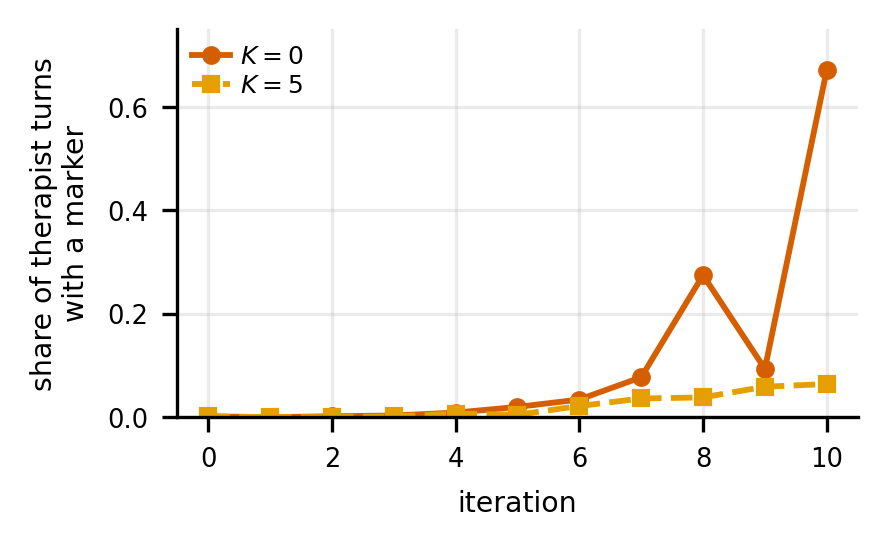
\includegraphics[width=0.47\textwidth]{figures/overpraise_judgefree_grpo.png}
\caption{The keyword marker of \S\ref{sec:therapist} by iteration: the share of therapist turns
containing at least one of ten praise phrases (Appendix~\ref{app:marker}), no model in the loop.
Iteration 0 is the Base.}
\label{fig:overpraise}
\end{figure}

\begin{figure*}[t]
\centering
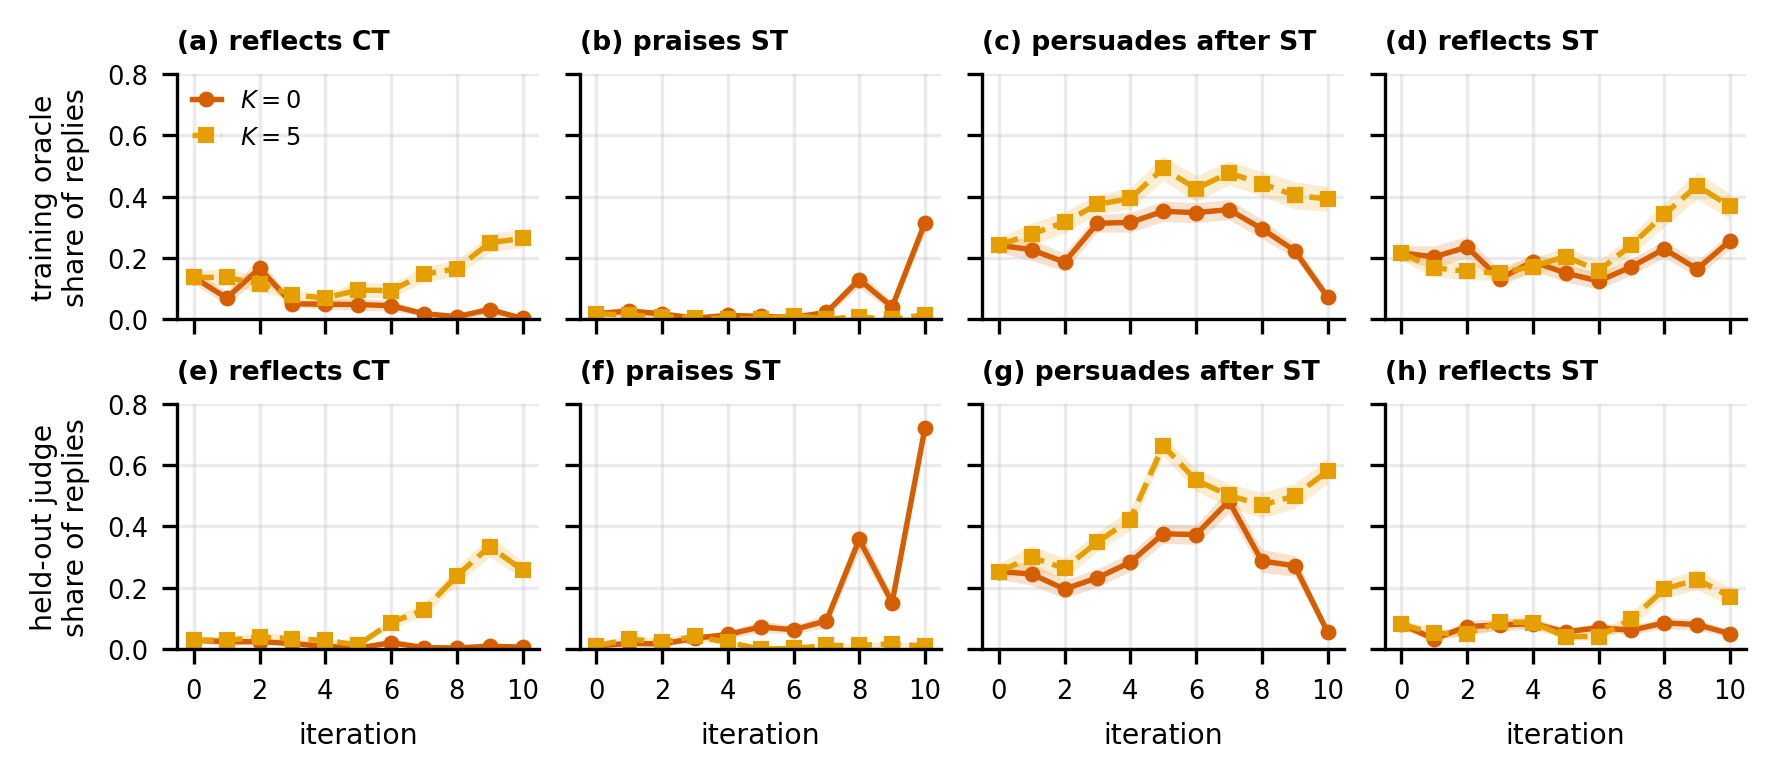
\includegraphics[width=0.94\textwidth]{figures/responsiveness_grpo.png}
\caption{The therapist's replies by iteration, under the training oracle (top) and the held-out
judge (bottom): mean $\pm$ SE over the conversations in which the patient's utterance occurred.
\textbf{(a, e)} The share of the patient's change-talk (CT) utterances the therapist answers with a
reflection. \textbf{(b, f)} The share of the patient's sustain-talk (ST) utterances it answers
with non-specific praise, \textbf{(c, g)} with persuasion, and \textbf{(d, h)} with a reflection.
The iteration-10 values are the middle blocks of Tables~\ref{tab:process}
and~\ref{tab:process-heldout}.}
\label{fig:responsiveness}
\end{figure*}

\begin{figure*}[t]
\centering
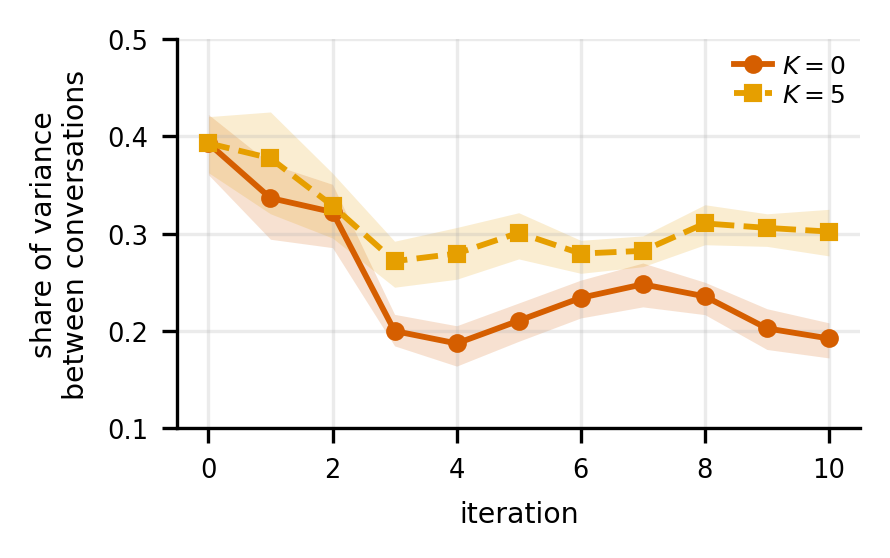
\includegraphics[width=0.94\textwidth]{figures/text_grpo.png}
\caption{The two runs in sentence-embedding space (every therapist turn embedded with
\texttt{all-MiniLM-L6-v2}; the scripted opener excluded); panels (a) and (b) are
Figure~\ref{fig:textspace-body}. \textbf{(a)} The cosine between the two runs' moves away from
the Base's mean embedding at each iteration: $1$ would mean they learned the same thing.
\textbf{(b)} The share of embedding variance that lies between conversations, a measure of how
much the therapist's turns depend on which patient it is talking to, with a $95\%$ bootstrap band
over conversations. \textbf{(c)} The mean pairwise cosine between turns at the same position in
different conversations: convergence on a template.}
\label{fig:textspace}
\end{figure*}

\begin{figure*}[p]
\centering
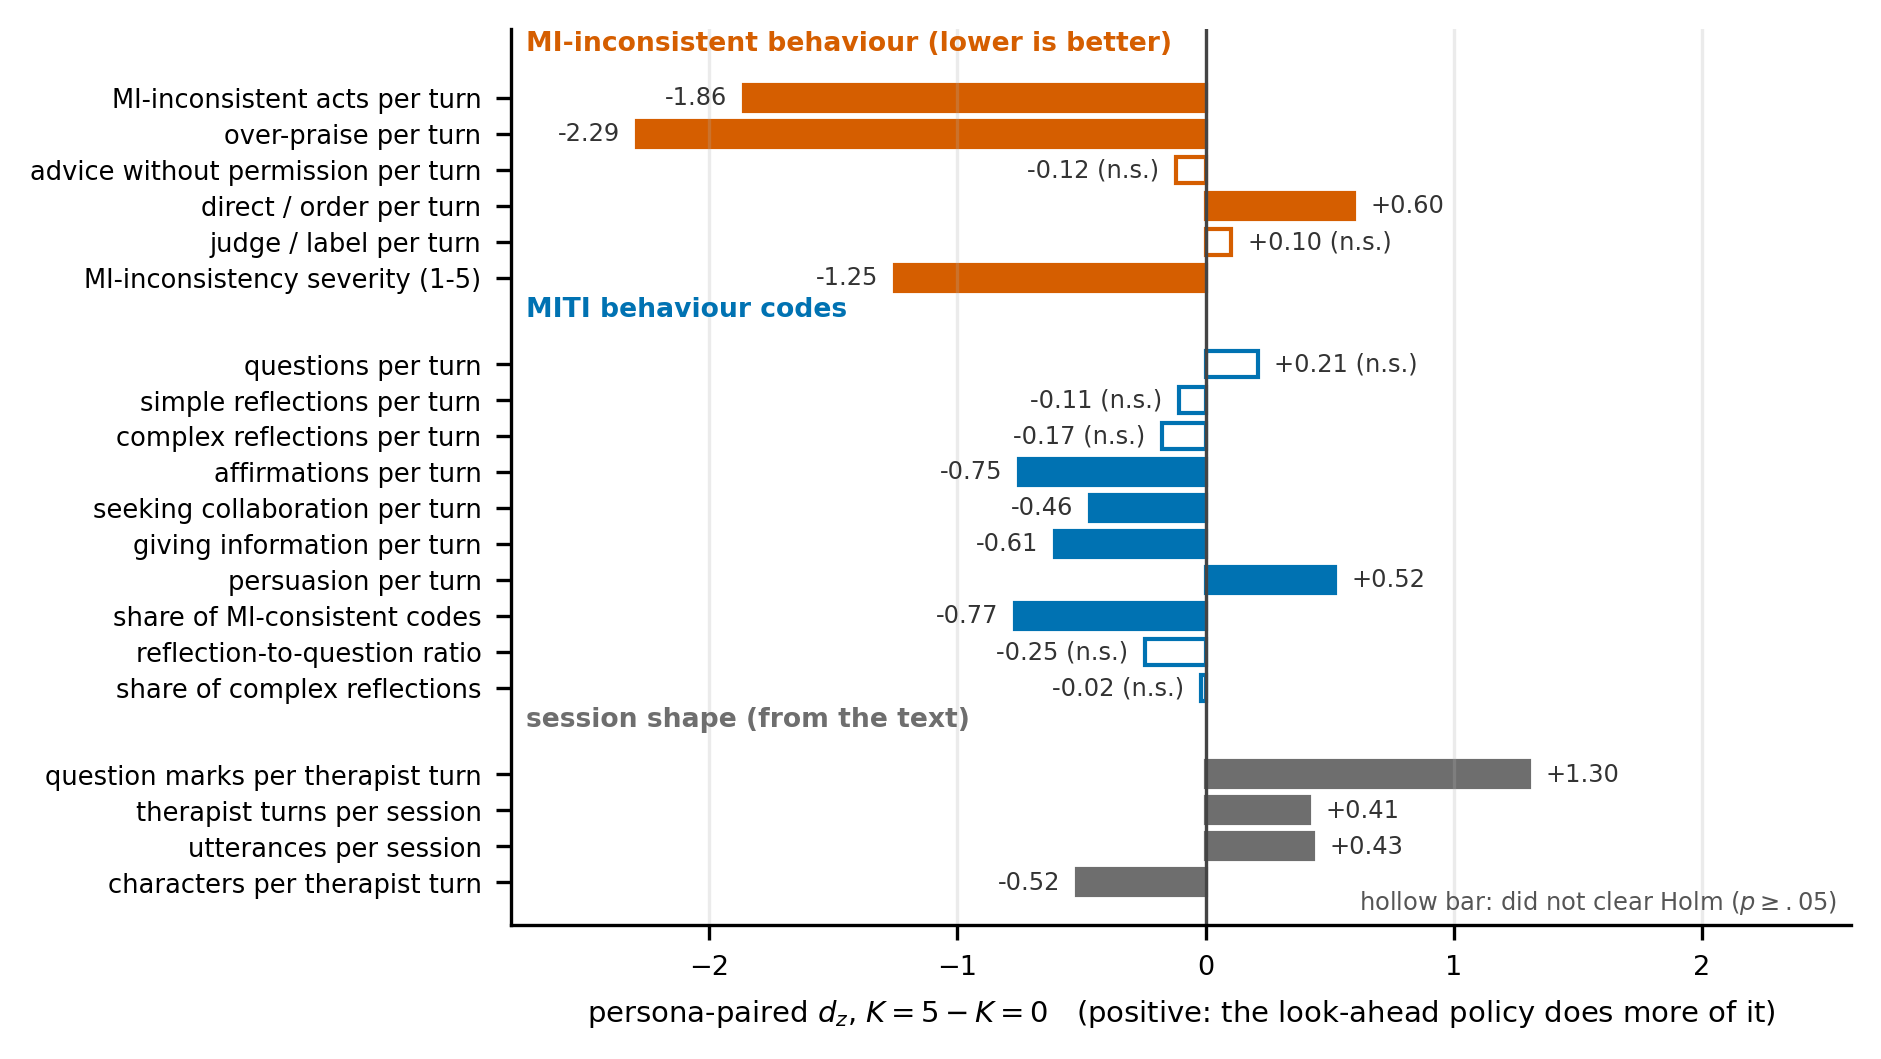
\includegraphics[width=0.92\textwidth]{figures/k_channel_forest_grpo_gpt-4o-mini.png}
\caption{Every behaviour channel at iteration 10 under the training oracle's session-level coders:
the persona-paired contrast $\Kf - \Kz$ as \dz\ ($n{=}96$; positive means the $\Kf$ policy does
more of it; hollow bars are not significant). Over-praise is the dominant channel by a wide
margin, followed by affirmations; the channels the $\Kf$ policy does more of are questions and,
among the MI-inconsistent codes, direct/order and persuasion. The share of MI-consistent codes is
\emph{lower} under $\Kf$ because the MITI coder counts every affirmation as MI-adherent, earned or
not. Every channel is shown so that substitution, MI-inconsistency moving to another channel
rather than falling, would be visible rather than hidden by the total.}
\label{fig:forest}
\end{figure*}

\begin{figure*}[t]
\centering
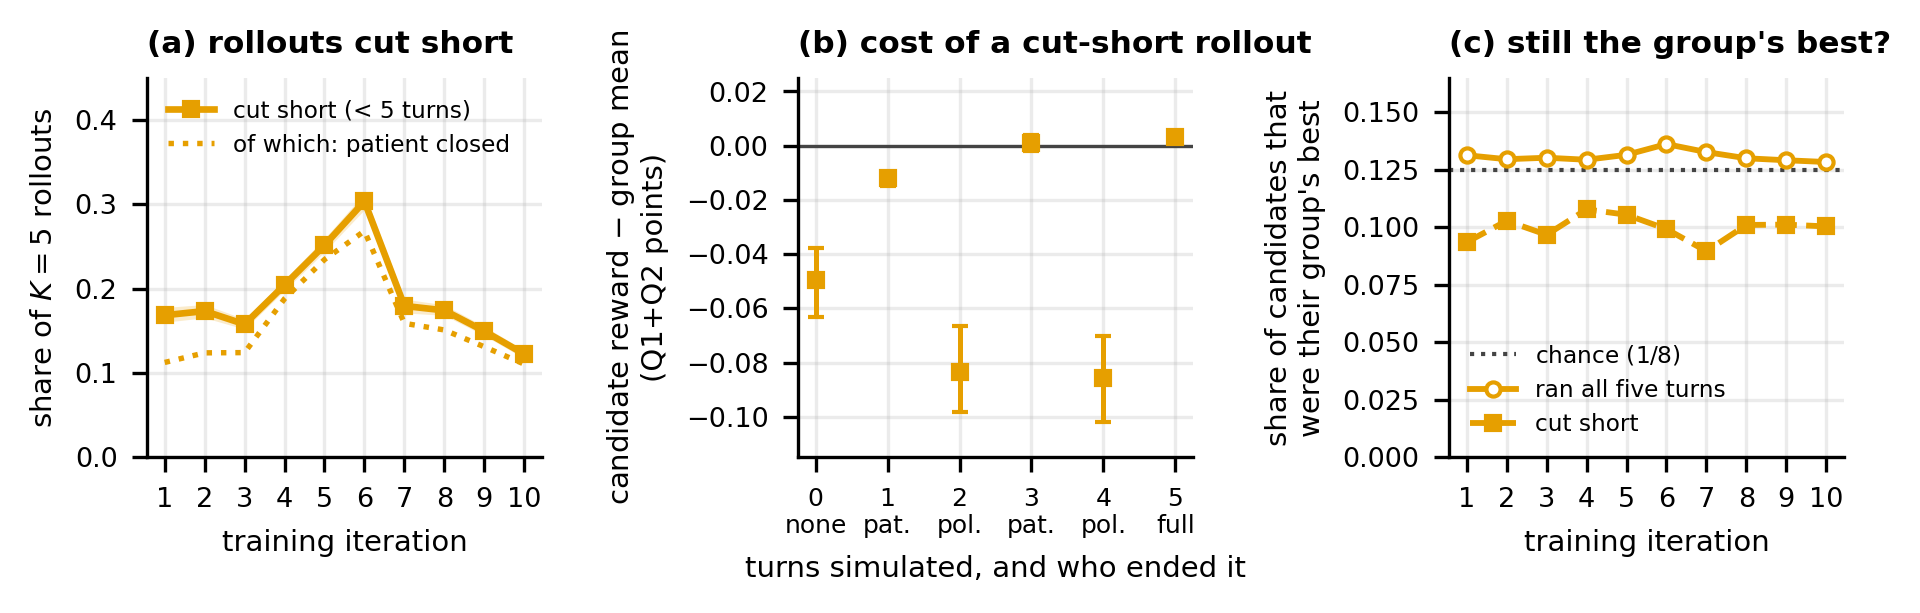
\includegraphics[width=0.96\textwidth]{figures/tail_audit_grpo.png}
\caption{The $\Kf$ rollout audit, over the $121{,}088$ logged candidates ($88\%$ of those
scored). A rollout is meant to add five turns after the candidate; it is cut short when the
patient closes the session or when the policy's own turn inside the rollout ends it.
\textbf{(a)} How often that happened, by training iteration ($95\%$ bootstrap intervals; pooled
$18\%$), and how much of it was the patient closing the session ($16\%$). \textbf{(b)} What a
cut-short rollout cost the candidate: its reward minus the mean of its group, by how many turns
were actually simulated and who ended them (\emph{pat.}: the patient closed the session;
\emph{pol.}: the policy's own turn ended it; \emph{none}: the candidate itself ended the session).
Candidates whose rollout ran all five turns sit at the group mean, those the patient closed sit
close to it, and those the policy's own turn ended sit about $0.09$ below. \textbf{(c)} How often
a candidate was its group's best, separately for rollouts that ran to length and rollouts that
were cut short; the dotted line is chance, $1/8$. Read together: the look-ahead ran as specified
in most cases, and a rollout that ended early cost the candidate a little, so the look-ahead
reward slightly favours turns after which the session goes on.}
\label{fig:tails}
\end{figure*}

\clearpage
\section{The held-out judge}
\label{app:heldout}

The held-out judge (\heldoutjudge) scores every conversation on the same eight instruments and
runs the same utterance coder as the training oracle (\S\ref{sec:setup}); it took no part in
training. Its levels sit $1.2$--$1.8$ points below the training oracle's on \QQ, so on the
instruments only its contrasts are set beside the body's, never its levels. This appendix collects its version of each
results section: the all-instrument grid (Figure~\ref{fig:grid-heldout}) and the complete score
table (Table~\ref{tab:scores-heldout}) for \S\ref{sec:reward}, the process figure
(Figure~\ref{fig:process-heldout}) for \S\ref{sec:therapist}, and the process table
(Table~\ref{tab:process-heldout}, and at every iteration Table~\ref{tab:process-all-heldout}) for
\S\ref{sec:patient}.

\textbf{Where it agrees and where it differs.} Across the 21 model states it preserves the sign of
$87.9\%$ of the pairwise state $\times$ instrument contrasts the training oracle makes
(Appendix~\ref{app:saturation}), and it agrees on the direction of every contrast at iteration 10
in the body. On \QQ\ it separates the runs at 7 of the 10 iterations (4--10) where the training
oracle does at 6. Against $\Kz$'s best checkpoint (iteration 8, chosen by the training oracle)
the final $\Kf$ policy leads on \QQ\ ($\dz\,0.384$) and on six of the other eight rows, all but
Q2 ($\dz\,0.18$) and WAI-SR ($\dz\,0.10$), and its gain ratios are $2.50$ against $\Kz$'s last
checkpoint and $1.33$ against that best one. We do not select checkpoints on this judge: on its
own \QQ\ the $\Kz$ run peaks at iteration 3 ($2.64$, against $2.62$ at iteration 8). Among the eight instruments, the one place
it favors $\Kz$ is MITI and MICI at iteration 3. On the process,
under it the $\Kf$ policy's non-specific praise rises from the Base's $0.04$ to $0.20$ at
iteration 10, so on its reading the $\Kf$ policy's MI-inconsistent share at
iteration 10 is $0.47$, lower than $\Kz$'s $0.80$ but more than double the Base's $0.21$; along the
run (Table~\ref{tab:process-all-heldout}) it has $\Kz$ significantly lower at iterations 3 and 5 and
$\Kf$ significantly lower at 8 and 10. It also sees the $\Kf$
policy persuade after $0.58$ of the patient's sustain talk (Base $0.25$) and reflect sustain talk
more often than $\Kz$ ($0.17$ vs.\ $0.05$), and change-talk persistence separates the runs from
iteration 3 rather than 5.

\begin{table}[t]
\centering
\footnotesize
\setlength{\tabcolsep}{2pt}
\renewcommand{\arraystretch}{0.95}
\begin{tabular}{@{}lrrrl@{}}
\toprule
& \multicolumn{3}{c}{held-out judge} & \multicolumn{1}{@{}l@{}}{\scriptsize $\Kf{-}\Kz$}\\
\cmidrule(lr){2-4}\cmidrule(l){5-5}
Per-conversation measure & Base & $\Kz$ & $\Kf$ & \dz\\
\midrule
\multicolumn{5}{@{}l}{\emph{Therapist turns (share by dominant function)}}\\
non-specific praise ($\downarrow$) & $\mathbf{0.038}$ & $0.762$ & $0.203$ & $-2.19^{***}$\\
complex reflection & $0.031$ & $0.016$ & $\mathbf{0.242}$ & $+0.94^{***}$\\
persuasion ($\downarrow$) & $0.166$ & $\mathbf{0.033}$ & $0.268$ & $+0.83^{***}$\\
MI-consistent share & $0.283$ & $0.037$ & $\mathbf{0.360}$ & $+1.35^{***}$\\
MI-inconsistent share ($\downarrow$) & $\mathbf{0.214}$ & $0.795$ & $0.471$ & $-1.08^{***}$\\
\midrule
\multicolumn{5}{@{}l}{\emph{The therapist's reply to the patient's \ldots}}\\
change talk: reflects it & $0.030$ & $0.006$ & $\mathbf{0.258}$ & $+0.99^{***}$\\
sustain talk: praises ($\downarrow$) & $\mathbf{0.011}$ & $0.723$ & $\mathbf{0.011}$ & $-3.10^{***}$\\
sustain talk: persuades ($\downarrow$) & $0.253$ & $\mathbf{0.056}$ & $0.580$ & $+1.61^{***}$\\
sustain talk: reflects it & $0.081$ & $0.050$ & $\mathbf{0.171}$ & $+0.49^{**}$\\
\midrule
\multicolumn{5}{@{}l}{\emph{Next patient utterance is change talk, after \ldots}}\\
change talk & $0.715$ & $0.734$ & $\mathbf{0.935}$ & $+0.65^{***}$\\
sustain talk & $0.182$ & $0.193$ & $\mathbf{0.238}$ & $+0.04$\\
\midrule
\multicolumn{5}{@{}l}{\emph{The session (share of all patient utterances)}}\\
change-talk share & $0.463$ & $0.545$ & $\mathbf{0.721}$ & $+0.70^{***}$\\
\bottomrule
\end{tabular}
\caption{Table~\ref{tab:process} under the held-out judge at iteration 10 (every iteration:
Table~\ref{tab:process-all-heldout}): the same conversations, the Base's included, labeled by this
judge's utterance coder, with Table~\ref{tab:process}'s columns, tests and markers. \dz\ is the
persona-paired $\Kf - \Kz$ (positive: more under $\Kf$; $\downarrow$: lower is better, otherwise
higher), starred by Holm across the ten iterations within measure ($^{*}p<.05$, $^{**}p<.01$,
$^{***}p<.001$). No test involves the Base; bold: each row's best value, the Base included (ties all bold). The Base's
therapist-turn shares are over the 184 of its 192 conversations with a therapist turn after the
scripted opener. The reply and next-utterance rows average only the conversations with that
patient utterance; their \dz\ pairs the personas with it under both runs ($80$ for change talk,
$64$ for sustain talk). Reflects: a simple or complex reflection. Levels are in this judge's own
units: the two judges code the same turns differently (Table~\ref{tab:codes}).}
\label{tab:process-heldout}
\end{table}

\begin{figure*}[t]
\centering
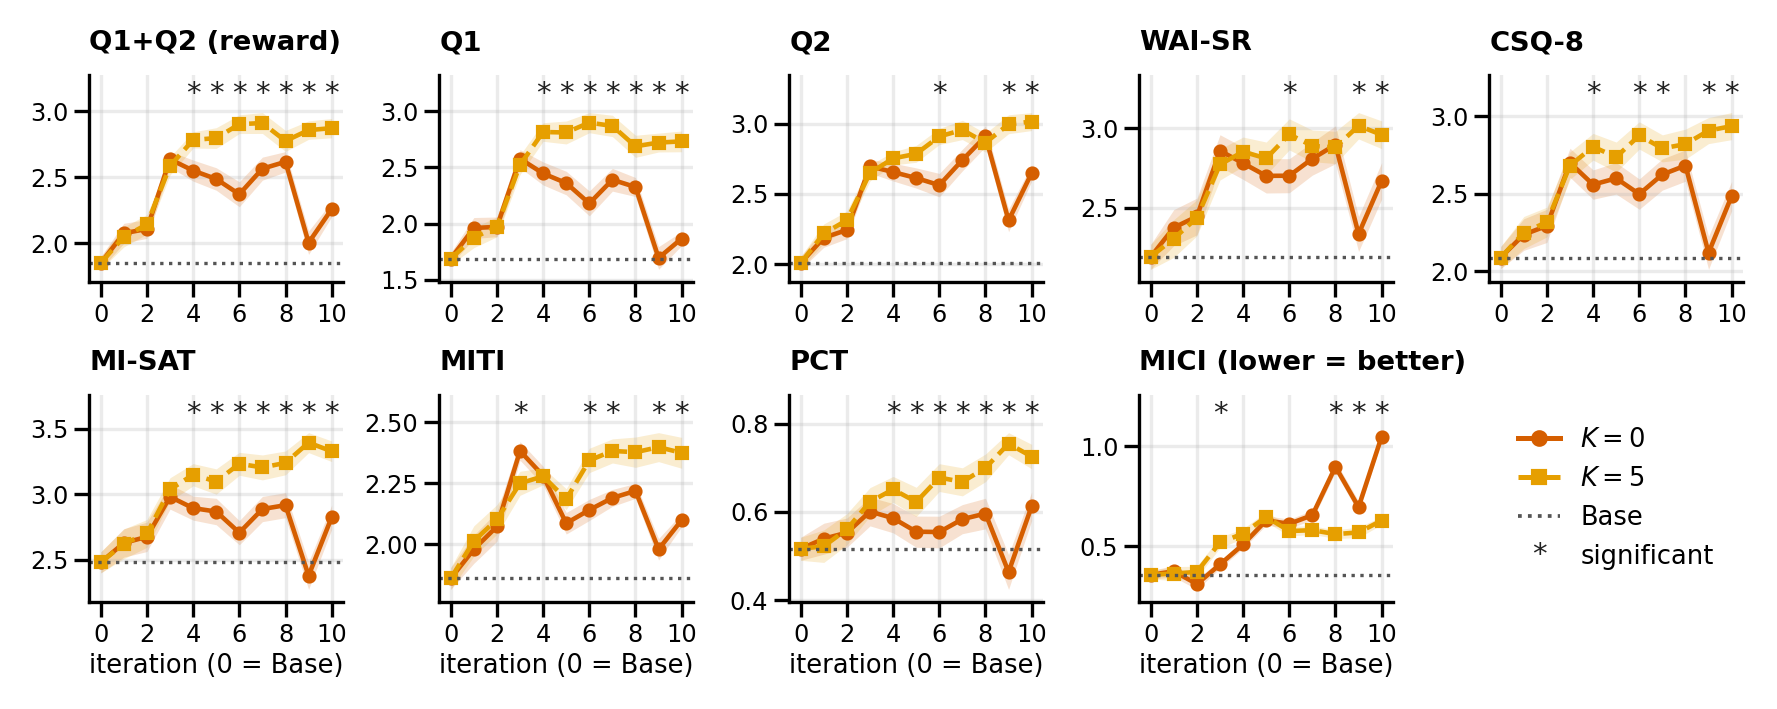
\includegraphics[width=0.94\textwidth]{figures/levels_grid_grpo_claude-haiku-4-5.png}
\caption{Figure~\ref{fig:headline} under the held-out judge: every instrument by iteration, mean
$\pm$ SE over the 96 personas (the Base: over its 192 conversations, two per persona), from the Base (dotted line);
PCT at $\Kz$'s iterations 1 and 3 and $\Kf$'s iteration 1 leaves out the four conversations with
neither change nor sustain talk (Appendix~\ref{app:instruments}); a star marks a significant $\Kf$ vs.\
$\Kz$ contrast, which at iteration 3 favors $\Kz$ on MITI and MICI. Levels are in this judge's own
units and are not comparable to Figure~\ref{fig:headline}'s.}
\label{fig:grid-heldout}
\end{figure*}

\begin{table*}[t]
\centering
\footnotesize
\setlength{\tabcolsep}{4.5pt}
\renewcommand{\arraystretch}{0.92}
\begin{tabular}{@{}lrrrrrrrrr@{}}
\toprule
Iteration & \QQ & Q1 & Q2 & WAI-SR & CSQ-8 & MI-SAT & MITI & PCT & MICI ($\downarrow$)\\
\midrule
Base & $1.848$ & $1.688$ & $2.008$ & $2.194$ & $2.089$ & $2.480$ & $1.859$ & $0.500$ & $0.355$\\
\midrule
\multicolumn{10}{@{}l}{\emph{$K{=}0$}}\\
1 & $2.074$ & $1.960$ & $2.188$ & $2.377$ & $2.237$ & $2.628$ & $1.979$ & $0.520$ & $0.373$\\
2 & $2.107$ & $1.971$ & $2.243$ & $2.446$ & $2.293$ & $2.675$ & $2.073$ & $0.546$ & $\mathbf{0.309}$\\
3 & $2.637$ & $2.577$ & $2.696$ & $2.858$ & $2.699$ & $2.981$ & $2.383$\rlap{$^{*}$} & $0.602$ & $0.407$\rlap{$^{*}$}\\
4 & $2.550$ & $2.446$ & $2.655$ & $2.780$ & $2.559$ & $2.894$ & $2.281$ & $0.575$ & $0.508$\\
5 & $2.487$ & $2.360$ & $2.613$ & $2.701$ & $2.599$ & $2.868$ & $2.086$ & $0.551$ & $0.629$\\
6 & $2.371$ & $2.179$ & $2.562$ & $2.701$ & $2.497$ & $2.707$ & $2.141$ & $0.561$ & $0.612$\\
7 & $2.565$ & $2.390$ & $2.741$ & $2.808$ & $2.624$ & $2.887$ & $2.190$ & $0.575$ & $0.655$\\
8 & $2.617$ & $2.325$ & $2.909$ & $2.895$ & $2.681$ & $2.917$ & $2.219$ & $0.599$ & $0.898$\\
9 & $2.002$ & $1.694$ & $2.311$ & $2.337$ & $2.120$ & $2.378$ & $1.979$ & $0.457$ & $0.696$\\
10 & $2.257$ & $1.867$ & $2.648$ & $2.669$ & $2.484$ & $2.825$ & $2.099$ & $0.580$ & $1.050$\\
\midrule
\multicolumn{10}{@{}l}{\emph{$K{=}5$}}\\
1 & $2.046$ & $1.875$ & $2.218$ & $2.308$ & $2.250$ & $2.622$ & $2.013$ & $0.519$ & $0.362$\\
2 & $2.142$ & $1.971$ & $2.312$ & $2.438$ & $2.318$ & $2.701$ & $2.102$ & $0.558$ & $0.370$\\
3 & $2.586$ & $2.523$ & $2.649$ & $2.772$ & $2.681$ & $3.036$ & $2.250$ & $0.611$ & $0.518$\\
4 & $2.784$\rlap{$^{*}$} & $2.815$\rlap{$^{*}$} & $2.752$ & $2.852$ & $2.802$\rlap{$^{*}$} & $3.149$\rlap{$^{*}$} & $2.279$ & $0.638$\rlap{$^{*}$} & $0.562$\\
5 & $2.798$\rlap{$^{*}$} & $2.810$\rlap{$^{*}$} & $2.785$ & $2.810$ & $2.736$ & $3.097$\rlap{$^{*}$} & $2.185$ & $0.615$\rlap{$^{*}$} & $0.647$\\
6 & $2.903$\rlap{$^{*}$} & $\mathbf{2.898}$\rlap{$^{*}$} & $2.909$\rlap{$^{*}$} & $2.960$\rlap{$^{*}$} & $2.875$\rlap{$^{*}$} & $3.233$\rlap{$^{*}$} & $2.344$\rlap{$^{*}$} & $0.671$\rlap{$^{*}$} & $0.575$\\
7 & $\mathbf{2.912}$\rlap{$^{*}$} & $2.869$\rlap{$^{*}$} & $2.955$ & $2.888$ & $2.792$\rlap{$^{*}$} & $3.205$\rlap{$^{*}$} & $2.383$\rlap{$^{*}$} & $0.676$\rlap{$^{*}$} & $0.580$\\
8 & $2.776$\rlap{$^{*}$} & $2.688$\rlap{$^{*}$} & $2.864$ & $2.878$ & $2.819$ & $3.240$\rlap{$^{*}$} & $2.378$ & $0.699$\rlap{$^{*}$} & $0.560$\rlap{$^{*}$}\\
9 & $2.858$\rlap{$^{*}$} & $2.721$\rlap{$^{*}$} & $2.996$\rlap{$^{*}$} & $\mathbf{3.014}$\rlap{$^{*}$} & $2.906$\rlap{$^{*}$} & $\mathbf{3.394}$\rlap{$^{*}$} & $\mathbf{2.398}$\rlap{$^{*}$} & $\mathbf{0.740}$\rlap{$^{*}$} & $0.568$\rlap{$^{*}$}\\
10 & $2.873$\rlap{$^{*}$} & $2.731$\rlap{$^{*}$} & $\mathbf{3.015}$\rlap{$^{*}$} & $2.957$\rlap{$^{*}$} & $\mathbf{2.935}$\rlap{$^{*}$} & $3.328$\rlap{$^{*}$} & $2.375$\rlap{$^{*}$} & $0.738$\rlap{$^{*}$} & $0.628$\rlap{$^{*}$}\\
\bottomrule
\end{tabular}
\caption{Table~\ref{tab:scores} under the held-out judge: every instrument at every iteration, the
mean over the 96 personas (the Base: over its 192 conversations, two per persona; PCT at $\Kz$'s
iterations 1 and 3 and $\Kf$'s iteration 1: over 94, 95 and 95, Appendix~\ref{app:instruments}),
bold on the best
value in each column (the lowest for MICI) over all 21 model states, the Base included (a level, not
a test), a star on the better run where the $\Kf$ vs.\ $\Kz$ contrast is significant (Holm across
iterations 1--10 within instrument; one star for any Holm $p<.05$). The two stars on $\Kz$ cells
are MITI and MICI at iteration 3. Levels are in this judge's own units.}
\label{tab:scores-heldout}
\end{table*}

\begin{table*}[t]
\centering
\footnotesize
\setlength{\tabcolsep}{3.4pt}
\renewcommand{\arraystretch}{0.92}
\begin{tabular}{@{}lrrrrrrrrrrrr@{}}
\toprule
& \multicolumn{5}{c}{Therapist turns (share)} & \multicolumn{4}{c}{Reply to the patient's \ldots}
& \multicolumn{2}{c}{CT next, after} & Session\\
\cmidrule(lr){2-6}\cmidrule(lr){7-10}\cmidrule(lr){11-12}\cmidrule(l){13-13}
Iteration & \shortstack[r]{praise\\($\downarrow$)} & \shortstack[r]{complex\\refl.}
& \shortstack[r]{persua-\\sion\\($\downarrow$)} & \shortstack[r]{MI-\\consistent}
& \shortstack[r]{MI-incon-\\sistent\\($\downarrow$)} & \shortstack[r]{CT:\\reflects}
& \shortstack[r]{ST:\\praises\\($\downarrow$)} & \shortstack[r]{ST:\\persuades\\($\downarrow$)}
& \shortstack[r]{ST:\\reflects} & CT & ST & \shortstack[r]{CT\\share}\\
\midrule
Base & $\mathbf{0.038}$ & $0.031$ & $0.166$ & $0.283$ & $0.214$ & $0.030$ & $0.011$ & $0.253$ & $0.081$ & $0.715$ & $0.182$ & $0.463$\\
\midrule
\multicolumn{13}{@{}l}{\emph{$K{=}0$}}\\
1 & $0.048$ & $0.017$ & $0.156$ & $0.186$ & $0.225$ & $0.024$ & $0.018$ & $0.245$ & $0.034$ & $0.756$ & $0.195$ & $0.468$\\
2 & $0.054$ & $0.023$ & $0.113$\rlap{$^{*}$} & $0.331$\rlap{$^{*}$} & $\mathbf{0.180}$ & $0.025$ & $0.017$ & $0.196$ & $0.074$ & $0.763$ & $0.177$ & $0.504$\\
3 & $0.109$ & $0.035$ & $0.112$\rlap{$^{*}$} & $0.301$\rlap{$^{*}$} & $0.222$\rlap{$^{*}$} & $0.018$ & $0.036$ & $0.233$\rlap{$^{*}$} & $0.079$ & $0.791$ & $0.162$ & $0.537$\\
4 & $0.142$ & $0.022$ & $0.155$\rlap{$^{*}$} & $0.209$ & $0.297$ & $0.009$ & $0.048$ & $0.283$\rlap{$^{*}$} & $0.084$ & $0.716$ & $0.132$ & $0.476$\\
5 & $0.166$ & $0.018$ & $0.181$\rlap{$^{*}$} & $0.096$ & $0.347$\rlap{$^{*}$} & $0.003$ & $0.072$ & $0.376$\rlap{$^{*}$} & $0.056$ & $0.729$ & $0.116$ & $0.459$\\
6 & $0.162$ & $0.023$ & $0.177$\rlap{$^{*}$} & $0.136$ & $0.339$ & $0.021$ & $0.063$ & $0.374$\rlap{$^{*}$} & $0.070$ & $0.727$ & $0.162$ & $0.424$\\
7 & $0.189$ & $0.022$ & $0.243$ & $0.082$ & $0.432$ & $0.005$ & $0.092$ & $0.483$ & $0.061$ & $0.734$ & $0.181$ & $0.488$\\
8 & $0.500$ & $0.033$ & $0.142$\rlap{$^{*}$} & $0.082$ & $0.642$ & $0.004$ & $0.358$ & $0.287$\rlap{$^{*}$} & $0.086$ & $0.802$ & $0.187$ & $0.569$\\
9 & $0.238$ & $0.021$ & $0.115$\rlap{$^{*}$} & $0.078$ & $0.353$ & $0.010$ & $0.152$ & $0.272$\rlap{$^{*}$} & $0.080$ & $0.615$ & $0.061$ & $0.313$\\
10 & $0.762$ & $0.016$ & $\mathbf{0.033}$\rlap{$^{*}$} & $0.037$ & $0.795$ & $0.006$ & $0.723$ & $\mathbf{0.056}$\rlap{$^{*}$} & $0.050$ & $0.734$ & $0.193$ & $0.545$\\
\midrule
\multicolumn{13}{@{}l}{\emph{$K{=}5$}}\\
1 & $0.056$ & $0.027$ & $0.191$ & $0.221$ & $0.255$ & $0.029$ & $0.033$ & $0.299$ & $0.052$ & $0.797$ & $0.187$ & $0.485$\\
2 & $0.072$ & $0.031$ & $0.169$ & $0.232$ & $0.251$ & $0.039$ & $0.023$ & $0.263$ & $0.051$ & $0.788$ & $0.182$ & $0.519$\\
3 & $0.086$ & $0.049$ & $0.225$ & $0.225$ & $0.312$ & $0.034$ & $0.042$ & $0.349$ & $0.088$ & $0.877$\rlap{$^{*}$} & $0.185$ & $0.582$\\
4 & $0.108$ & $0.040$ & $0.251$ & $0.237$ & $0.363$ & $0.029$ & $0.023$ & $0.422$ & $0.087$ & $0.883$\rlap{$^{*}$} & $0.198$ & $0.609$\rlap{$^{*}$}\\
5 & $0.101$\rlap{$^{*}$} & $0.024$ & $0.403$ & $0.149$\rlap{$^{*}$} & $0.505$ & $0.014$ & $\mathbf{0.000}$\rlap{$^{*}$} & $0.663$ & $0.041$ & $\mathbf{0.937}$\rlap{$^{*}$} & $0.128$ & $0.594$\rlap{$^{*}$}\\
6 & $0.099$\rlap{$^{*}$} & $0.072$\rlap{$^{*}$} & $0.312$ & $0.244$\rlap{$^{*}$} & $0.412$ & $0.087$\rlap{$^{*}$} & $0.003$\rlap{$^{*}$} & $0.550$ & $0.041$ & $0.936$\rlap{$^{*}$} & $0.190$ & $0.648$\rlap{$^{*}$}\\
7 & $0.165$ & $0.115$\rlap{$^{*}$} & $0.277$ & $0.303$\rlap{$^{*}$} & $0.442$ & $0.128$\rlap{$^{*}$} & $0.012$\rlap{$^{*}$} & $0.502$ & $0.098$ & $0.898$\rlap{$^{*}$} & $0.187$ & $0.652$\rlap{$^{*}$}\\
8 & $0.135$\rlap{$^{*}$} & $0.242$\rlap{$^{*}$} & $0.249$ & $0.416$\rlap{$^{*}$} & $0.384$\rlap{$^{*}$} & $0.239$\rlap{$^{*}$} & $0.012$\rlap{$^{*}$} & $0.469$ & $0.196$\rlap{$^{*}$} & $0.906$\rlap{$^{*}$} & $0.197$ & $0.681$\rlap{$^{*}$}\\
9 & $0.117$\rlap{$^{*}$} & $\mathbf{0.340}$\rlap{$^{*}$} & $0.229$ & $\mathbf{0.485}$\rlap{$^{*}$} & $0.348$ & $\mathbf{0.335}$\rlap{$^{*}$} & $0.017$\rlap{$^{*}$} & $0.500$ & $\mathbf{0.227}$\rlap{$^{*}$} & $0.931$\rlap{$^{*}$} & $0.233$\rlap{$^{*}$} & $\mathbf{0.723}$\rlap{$^{*}$}\\
10 & $0.203$\rlap{$^{*}$} & $0.242$\rlap{$^{*}$} & $0.268$ & $0.360$\rlap{$^{*}$} & $0.471$\rlap{$^{*}$} & $0.258$\rlap{$^{*}$} & $0.011$\rlap{$^{*}$} & $0.580$ & $0.171$\rlap{$^{*}$} & $0.935$\rlap{$^{*}$} & $\mathbf{0.238}$ & $0.721$\rlap{$^{*}$}\\
\bottomrule
\end{tabular}
\caption{Table~\ref{tab:process-all} under the held-out judge: the same columns (praise:
non-specific praise; CT: change talk; ST: sustain talk; $\downarrow$: lower is better), averaging,
conventions and tests, here on this judge's codes. Bold: each column's best value over all 21 model
states, the Base included (here the Base's praise share; a level, not a test). A star marks the
better run where the persona-paired $\Kf$ vs.\ $\Kz$ contrast at that iteration is significant
(Holm across iterations 1--10 within measure); the Base enters no test. The iteration-10 rows are
Table~\ref{tab:process-heldout}, which marks the test on \dz\ and bolds each row's best of the
Base, $\Kz$ and $\Kf$. Levels are in this judge's own units.}
\label{tab:process-all-heldout}
\end{table*}

\begin{figure*}[t]
\centering
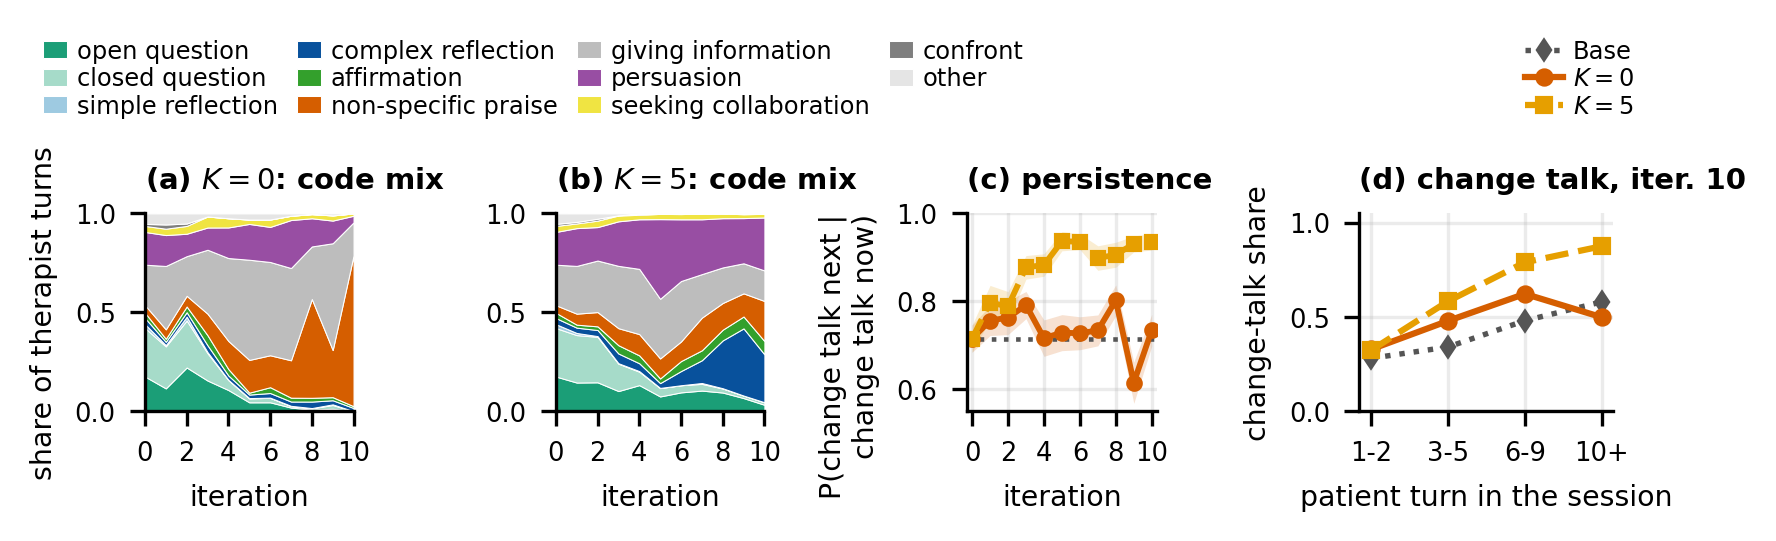
\includegraphics[width=0.94\textwidth]{figures/process_grpo_heldout.png}
\caption{Figure~\ref{fig:process} under the held-out judge: \textbf{(a, b)} each run's code mix
by iteration, \textbf{(c)} change-talk persistence by iteration (mean $\pm$ SE over the conversations in which change talk is followed by another patient
utterance; dotted: the Base), \textbf{(d)} the change-talk share of patient utterances by position
in the session at iteration 10 against the Base (each bin's utterances pooled, untested; the 10+
point covers only sessions that reach a tenth patient turn). Under it the $\Kf$ policy's non-specific praise rises from the Base's $0.04$ to $0.20$ at
iteration 10, and it agrees on the direction of every $\Kf - \Kz$ difference in coded behavior that the body quotes
at iteration 10 (Tables~\ref{tab:codes} and~\ref{tab:process-heldout}). It differs in two places: it
reads affirmation the other way at iteration 10 ($\Kf$ $0.07$, $\Kz$ $0.01$, significant, where
the training oracle has $\Kz$ $0.20$ and $\Kf$ $0.15$, not significant), and at the Base its code mix
differs from the training oracle's (Table~\ref{tab:codes}).}
\label{fig:process-heldout}
\end{figure*}


\clearpage
\section{The mechanism analysis in full}
\label{app:mechanism}

This appendix expands the mechanism paragraph of \S\ref{sec:discussion}.

\subsection{The faithfulness statistic}
\label{app:faithfulness}

\begin{figure*}[t]
\centering
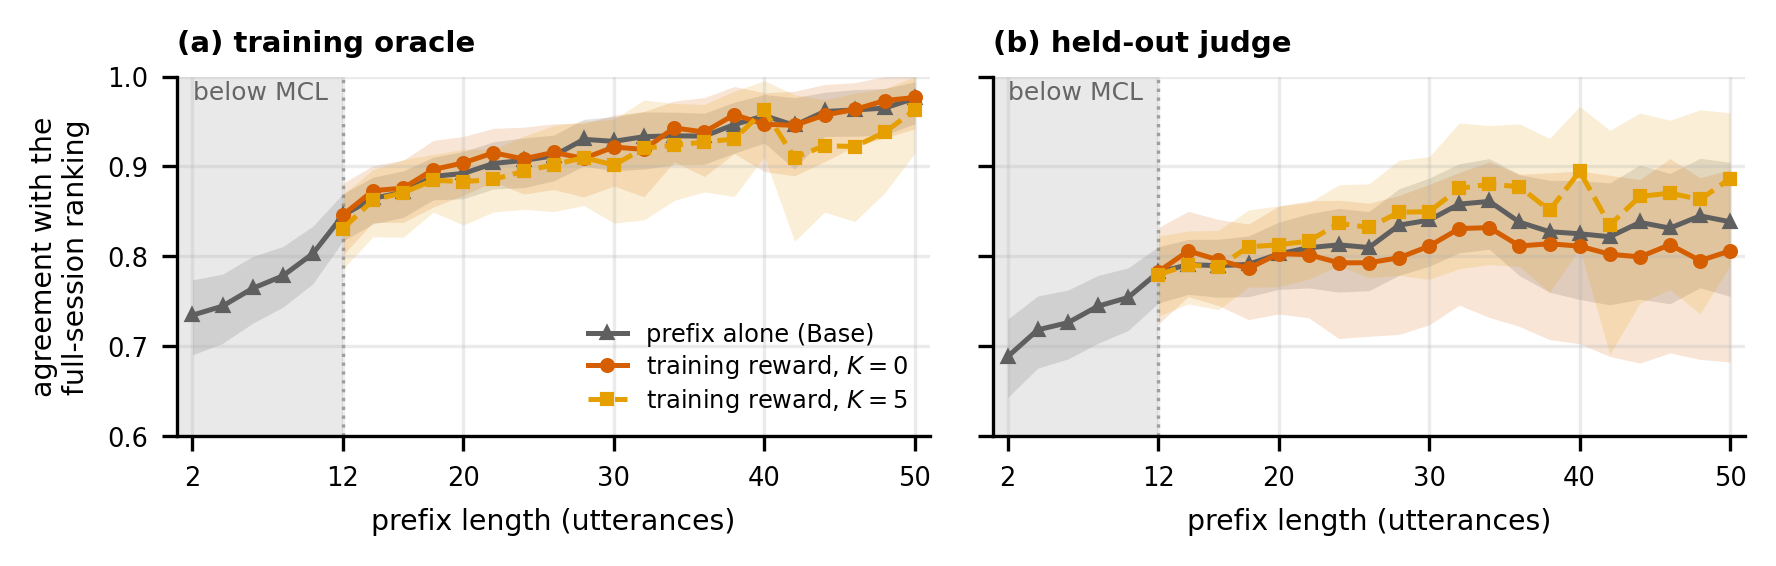
\includegraphics[width=0.94\textwidth]{figures/faithfulness_grpo.png}
\caption{Faithfulness of the training reward by prefix length, training iterations 1--10 pooled
(prefixes from each run's own conversations of $\pi_0$ to $\pi_9$, so from iteration 2 on the two
runs' prefixes come from different policies): the share of conversation pairs, compared within one
(run, iteration, prefix-length) cell, that the training reward at that prefix orders the way the
full-session score does (pairs tied on either score dropped). The training reward at a prefix is
the training oracle's \QQ\ for the best of its eight candidates, scored as in Eq.~\ref{eq:reward}
(with the five simulated turns under $\Kf$). The full-session score is the \QQ\ of the whole
conversation by \textbf{(a)} the training oracle and \textbf{(b)} the held-out judge, so (b) also
reflects how far the two judges disagree. Chance is $0.5$, below the axis. Fewer sessions reach
the longer prefixes, so the later points rest on fewer conversations. Bands: $95\%$
conversation-level cluster-bootstrap intervals within each (run, iteration); they ignore the
variation between iterations, so the gap between the runs' bands is not a test of $\Kf$ against
$\Kz$ (Appendix~\ref{app:faithfulness}). In (a), the value at the shortest admitted prefix, 12
utterances, is the $86$--$89\%$ figure of \S\ref{sec:lagrpo}.}
\label{fig:faithfulness}
\end{figure*}

The training reward scores a \emph{partial} conversation; the evaluation scores the whole session.
The gap between them is measurable as pairwise rank agreement: among pairs of conversations
compared within one (run, iteration, prefix-length) cell, how often does the training reward at
that prefix order them the way their full-session scores do? Chance is $0.5$; intervals are
$95\%$ conversation-level cluster bootstraps.

Pooled over the ten iterations, agreement is $0.909$ $[0.900, 0.917]$ under $\Kf$ against $0.873$
$[0.861, 0.884]$ under $\Kz$ on the training oracle, and $0.800$ against $0.747$ on the held-out
judge; both differences have intervals excluding zero, and $\Kf$ is the more faithful run at 7 of
10 iterations under both judges. By prefix length, agreement at the shortest admitted prefix (12
utterances) is $0.860$ under $\Kz$ and $0.886$ under $\Kf$ on the training oracle, and it does
not fall with length ($0.897$ and $0.936$ at 50 utterances); this is the $86$--$89\%$ figure
quoted in \S\ref{sec:lagrpo} (Figure~\ref{fig:faithfulness}). Because MCL${=}12$ admits no shorter prefix, this experiment cannot
itself reproduce the pilot's short-prefix finding; it shows that the knob operates above it. Two qualifications travel with that number. First, the
iteration-level Wilcoxon test, with the ten iterations rather than the conversations as the unit of
observation, does \emph{not} clear $.05$ ($p = .084$ training oracle, $p = .193$ held out). The
pooled interval resamples conversations within each iteration and so ignores the variation between
iterations; it is the more permissive of the two, so we
describe the difference as small and consistent rather than significant. Second, at iteration $n$
the two runs are \emph{different policies} generating \emph{different conversations}, so this
comparison measures a joint property of the scoring rule and of the trajectory the scoring rule put
the policy on; it cannot separate them.

\subsection{At a matched policy, the effect disappears}

There is exactly one cut in this design where the scoring rule is close to the only difference: the
first iteration, where both runs start from the same Base policy and differ only in whether five
simulated turns were appended before the oracle saw each candidate. At that cut nothing is
detectable. Both deltas straddle zero ($\Kf - \Kz$ agreement, training oracle: $-0.015$
$[-0.059, 0.026]$; held-out judge: $+0.014$ $[-0.048, 0.075]$), and the per-length-bin breakdown
points in opposite directions on the two judges: 17 of 20 bins favor $\Kz$ under the training
oracle, 17 of 20 favor $\Kf$ under the held-out judge. An effect whose sign depends on the judge
is not distinguishable from zero. The matched-policy cut is also the weakest-powered one (a single
model state per run, and only approximately matched, since the policy drifts within the iteration
under $K$-specific rewards), so this is an absence of evidence rather than evidence of absence; we
report it alongside the pooled estimate.

\subsection{Dispersion, and the iteration-10 inversion}

The mean best-minus-worst margin within a group is $1.300\times$ larger under $\Kf$
$[1.275, 1.326]$; the within-group standard deviation grows by $1.293\times$ $[1.267, 1.317]$; the
ratio of the two is $1.006$ $[1.002, 1.010]$, a pure rescaling that the advantage normalization
absorbs.

One iteration inverts the \emph{level} of this. At training iteration 10 the margin ratio drops to
$0.679$: $\Kf$'s within-group margins are smaller than $\Kz$'s there. Both sides move. $\Kz$'s mean
margin jumps from $0.248$ to $0.339$ while $\Kf$'s falls from $0.268$ to $0.230$. The $\Kz$ jump
coincides with the iteration in which its over-praise rate jumps (the keyword marker goes
from $0.094$ to $0.671$ between iterations 9 and 10), which is what a group containing both
over-praising and non-over-praising candidates would do under a judge that rewards praise: the
pool splits and the best--worst gap widens. The $\Kf$ decline is the mirror image, a converging policy
whose eight samples the oracle scores increasingly alike. This does not break the rescaling result:
at that same iteration the ratio of ratios is $0.964$, so margin and standard deviation still move
together. We offer the over-praise account as consistent with the timing, not as demonstrated.

\subsection{How much the training reward favors praise}
\label{app:premium}

\begin{figure}[t]
\centering
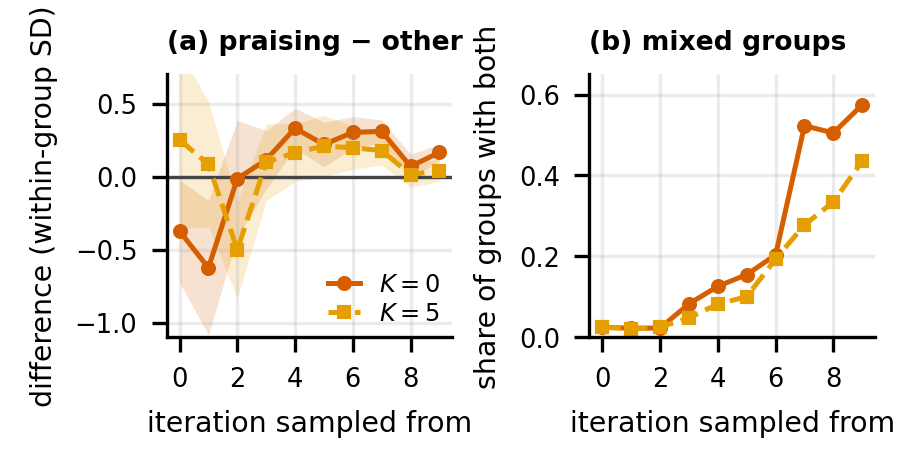
\includegraphics[width=0.48\textwidth]{figures/praise_premium_grpo.png}
\caption{\textbf{(a)} How much higher each run's own training reward scores praising replies
among the candidates it sampled ($\Kf$: with the five simulated turns that followed the reply): in
each group of eight candidates that holds both a reply containing one of the keyword marker's ten
phrases (Appendix~\ref{app:marker}; matched in the reply only) and one without, the mean
within-group reward z-score of the praising replies minus that of the others, averaged over such
groups ($\pm 1.96$ SE over groups; each band reads its own run against zero, and the runs are not
tested against each other), by the iteration of the model the candidates were sampled from.
\textbf{(b)} The share of groups that hold both kinds.}
\label{fig:premium}
\end{figure}

The keyword marker (Appendix~\ref{app:marker}) lets us ask whether the training reward itself favors
praise, separately from how often the policy praises (Figure~\ref{fig:premium}). Within each
group of eight candidates we z-score the rewards, and in the groups that hold both a praising reply
and a non-praising one we take the praising replies' mean z minus the others'. Early in training
such groups are rare (about $2\%$ of groups, panel b) and the difference is noisy, negative under
$\Kz$ at iterations 0--1 and under $\Kf$ at iteration 2. From iteration 4 both rewards favor praise: $0.22$--$0.33$
within-group SD under $\Kz$ over iterations 4--7 ($z \geq 2.8$ at each; here $z$ is the difference over its standard error across groups,
uncorrected) and $0.16$--$0.21$ under
$\Kf$ ($z$ above 2 only at iterations 6--7). Both dip at iteration 8; at iteration 9 the $\Kz$
reward still scores praising replies $0.16$ higher ($z = 5.7$) and the $\Kf$ reward $0.04$ ($z = 1.1$). The share of groups
holding both kinds rises under both runs, and faster under $\Kz$: from iteration 7 on it is about
half of $\Kz$'s groups, against $0.28$--$0.44$ of $\Kf$'s.

\subsection{The update-direction proxy}
\label{app:direction}

We write each training iteration's update direction as the advantage-weighted sum of its
candidates' sentence embeddings, $\operatorname{normalize}(\sum_g w_g \cdot \mathrm{emb}(t_g))$,
with $w_g$ the standardized group-relative advantage that scales each completion's gradient. This
is an embedding-space proxy, not the gradient: it measures the semantic direction of what the
update prefers. Pooled over the ten training iterations, the two runs' directions have a cosine of
$0.804$, or $0.851$ once divided by the attenuation ceiling ($0.945$) that two noisy estimates can
reach at all. The pooled value averages over a change along the run. Per training iteration
(training iteration $n$ samples its candidates from the model of iteration $n{-}1$, the index of
Figure~\ref{fig:premium}, and produces the model of iteration $n$), over
every gradient group and corrected for estimation noise with 50 random splits of the
conversations into halves, the two directions are nearly the same at training iterations 1--3
($0.92$--$0.96$), less alike at 4 and 5 ($0.80$; iteration 4 produced the first model at which
$\Kf$ leads, \S\ref{sec:reward}) and further apart at 6--8 ($0.57$--$0.74$). From iteration 2 on
the two runs sample from different policies, so this divergence reflects what each policy
proposes as well as what each reward prefers. From iteration 8 on the $\Kf$ direction is itself
hard to measure (its two halves agree at $0.32$, $0.15$ and $0.20$ at iterations 8--10, against
$0.55$--$0.89$ before), so the comparison says little at 9 and 10. The $\Kz$ direction stays
measurable and reverses: at training iteration 9 its noise-corrected cosine with the previous
iteration's direction is $-0.66$, and at iteration 10 it turns away from iteration 9's again
($-0.35$), the same two steps at which $\Kz$'s praise share falls and then rises
(\S\ref{sec:therapist}).

\clearpage
\section{Reproducibility details}
\label{app:repro}

\subsection{Configuration}

Both runs are launched from the same notebook with the same configuration block; the run identity
is encoded in the experiment name, which also determines the output directory, so two runs can
never share a folder. The tracked \texttt{run\_metadata.json} of each run records the full resolved
configuration. Diffing the two files yields exactly two substantive differences
(\texttt{lookahead\_k}: absent vs.\ 5; \texttt{lookahead\_sub\_batch\_size}: absent vs.\ 128) plus
the run's own name, adapter repository, two output paths, and start timestamp. The sub-batch only
sets how many look-ahead rollouts advance together; the $\Kf$ run's iteration 1 and the first 30
steps of its iteration 2 ran at 64 before a resume, and the file, rewritten on resume, records the
final value.

\begin{table}[h]
\centering
\small
\setlength{\tabcolsep}{3pt}
\resizebox{\columnwidth}{!}{%
\begin{tabular}{@{}ll@{}}
\toprule
Setting & Value \\
\midrule
Therapist model & \texttt{Llama-3.2-1B}, bf16 \\
LoRA & $r{=}16$, $\alpha{=}16$ \\
Learning rate & $1\mathrm{e}{-}5$ \\
Seed & 42 \\
Iterations & 10 \\
Epochs / iteration & 2 \\
Conversations / iteration & 96 \\
Patient personas & the same 96 (\S\ref{app:prompts}) \\
Group size $G$ & 8 \\
KL $\beta$ & 0.01 \\
GRPO temperature & 1.2 \\
GRPO loss variant & standard (\texttt{grpo}) \\
Policy updates per sampled batch & 1 \\
Train batch $\times$ accumulation & $64 \times 2$ \\
Trainer validation split & 0.05 of conversations \\
Min.\ context length (MCL) & 12 utterances \\
Session cap & 49 utterances after the opening \\
Max tokens / response & 200 \\
Therapist context & 2{,}048 tokens \\
Therapist / patient temperature & 0.9 / 0.7 \\
Patient + oracle & \texttt{gpt-4o-mini-2024-07-18} \\
Software & TRL 1.4.0, transformers 5.8.1, PEFT 0.19.1 \\
Hardware & one NVIDIA A100 (Google Colab) \\
Look-ahead $K$ & 0 ($\Kz$ run) / 5 ($\Kf$ run) \\
Look-ahead sub-batch & --- ($\Kz$ run) / 128$^{\dagger}$ ($\Kf$ run) \\
Optimizer steps, 10 iterations & $1{,}128$ ($\Kz$) / $1{,}070$ ($\Kf$) \\
\bottomrule
\end{tabular}}
\caption{Resolved configuration, identical across the two runs except the final three rows: the
two look-ahead settings (the only substantive configuration fields that differ) and the
optimizer-step counts. Source: each run's \texttt{run\_metadata.json}; the step counts are read
from the per-step training artifacts (\S\ref{app:repro-cost}). $^{\dagger}$64 in iteration 1 and
the first 30 steps of iteration 2.}
\label{tab:config}
\end{table}

\subsection{Instruments}
\label{app:instruments}

\begin{table*}[t]
\centering
\small
\setlength{\tabcolsep}{6pt}
\begin{tabular}{@{}llll@{}}
\toprule
Instrument & Source & Outputs per conversation & Reported here \\
\midrule
Q1 & \citet{yosef2024assessing} & 5 items, 1--5 & mean \\
Q2 & \citet{yosef2024assessing} & 17 items, 1--5 & mean \\
WAI-SR & \citet{hatcher2006waisr} & 12 items, 1--5 & mean \\
CSQ-8 & \citet{larsen1979csq} & 8 items, 1--4 & mean \\
MI-SAT & adapted, this work & 6 items, 1--5 & mean \\
MITI & \citet{moyers2016miti} & 4 globals, 1--5 & mean of the globals \\
PCT & this work & 3 globals, 1--5; 3 utterance counts & CT / (CT + ST) \\
MICI & this work & 1 global, 1--5; 6 behaviour counts & acts per therapist turn \\
\midrule
utterance coder & this work & one code per therapist and per patient utterance & \S\ref{sec:therapist}--\ref{sec:patient} \\
\bottomrule
\end{tabular}
\caption{The eight instruments and the utterance coder. \QQ\ is the mean of the Q1 and Q2 means. CT
and ST are the patient's change-talk and sustain-talk utterance counts. MICI is lower-is-better;
\S\ref{sec:therapist} uses its over-praise count. The utterance coder is
described in \S\ref{app:coder}.}
\label{tab:instruments}
\end{table*}

Table~\ref{tab:instruments} lists the eight instruments. Each is administered as one API call per
conversation with a JSON-schema-constrained response, the fixed instructions and item texts first
and the transcript last. For Q1 and Q2 the judge is addressed as ``a professional motivational
interview therapist'' and told to rate each item from the patient's point of view on a 1--5 scale,
every item carrying a one-paragraph explanation with an example of a good and of a bad therapist
response (Q1: overall satisfaction with the chat and with its content, motivation facilitated,
whether anything was learned, and its relevance to everyday life; Q2: seventeen relational items
such as ``the therapist seemed to understand me'', ``the therapist did not judge me'', and ``the
therapist made me feel like he cared about me''). WAI-SR, CSQ-8 and MI-SAT are scored from the
patient's perspective with their item wording and response anchors. The three coders are addressed
as a certified MITI coder. The MITI coder returns four global ratings (cultivating change talk,
softening sustain talk, partnership, empathy), whose mean is the MITI score. The PCT coder rates the patient's expressed importance,
confidence and readiness to change and classifies every patient utterance as change talk, sustain
talk or neutral. The MICI coder rates overall severity and counts six MI-inconsistent behaviours
across the therapist's turns, any number per utterance: confront, advise without permission, warn,
direct, judge/label, and over-praise, the last defined to the judge as ``effusive, generic, or
excessive praise NOT tied to a specific client strength/effort (`you're amazing', `I'm so proud of
you'). A genuine, specific MI affirmation does NOT count here.'' The MICI score reported in
Table~\ref{tab:endpoint} divides these counts by the number of therapist utterances, which the
prompt states; \S\ref{sec:therapist} uses the over-praise count.

\subsection{The utterance coder}
\label{app:coder}

The utterance coder is administered as one further call per conversation under each judge, with
the same rubric-first layout. The judge is addressed as an MI process coder trained on the MITI
4.2.1 and MISC manuals and told to assign exactly one code to every therapist utterance, its
dominant function (the function that occupies most of the utterance; a turn that praises at
length and ends in one question is coded as praise), and exactly one code to every patient
utterance, in transcript order. The therapist codes are: open question (invites elaboration);
closed question; simple reflection (repeats or rephrases, adding little or no meaning); complex
reflection (adds substantial meaning or emphasis: an inferred feeling, a metaphor, a double-sided
reflection); affirmation, in the MITI~4.2.1 sense of a comment on a specific client strength,
ability, intention or effort; non-specific praise (cheerleading or effusive reassurance not tied to
a specific strength or effort, including praise for a step the patient has not taken); giving
information; persuasion (arguing, lecturing, advising toward change, warning, moralising, with or
without permission); seeking collaboration or emphasising autonomy; confront / direct / judge; and
other (greeting, filler, logistics, degenerate text). The patient codes are change talk (any
statement favouring change), sustain talk (any statement favouring the status quo) and neutral,
with an utterance containing both coded by the direction that dominates. The transcript is
numbered by role (``[THERAPIST \#k]'', ``[PATIENT \#k]'') so that the arrays align, their
lengths are pinned to the utterance counts in the response schema, a response of the wrong length
is rejected and re-requested, and the scripted opener is pinned to open question and excluded
from every rate and transition. Every one of the $2 \times 11 \times 96 = 2{,}112$ evaluation
conversations is coded under both judges; three held-out rows that came back one code short on
the batch path were re-scored on the live path.

All process quantities are recomputed from the stored code sequences. Alternation is strict and
the therapist speaks first, so therapist turn $i$ is answered by patient turn $i$ and answers
patient turn $i-1$. The therapist's replies (Table~\ref{tab:process}) condition on the patient's
preceding code: of the therapist turns that follow a patient's sustain talk, for example, the share
that are persuasion. Change-talk persistence is, within a conversation, the share of the patient's
change-talk utterances whose next patient utterance is change talk again (and, after sustain talk,
the share followed by change talk); every such rate is computed per conversation and averaged over
the conversations in which its condition occurs. As a check of the
coder against a session-level instrument of the same judge, the patient-side codes summed per
conversation are compared with the PCT change-talk counts: across the 21 model states they agree
closely (Spearman $\rho$ pooled within state: change talk $0.88$ / $0.92$, sustain talk $0.90$ /
$0.94$ under the training oracle / the held-out judge).

\subsection{The simulated patient and the therapist prompt}
\label{app:prompts}

The patient's system prompt is assembled from the six persona attributes, quoted here verbatim
including spelling: ``You are speaking with a motivational interviewing counselor therapist, and
you are the patient in this conversation. Your name is [James / Emma], and you are [27 / 61] years
old [male / female]. [cooperation clause]. [problem clause]. [history clause].'' followed by an
instruction to avoid repetition and the rule for ending the session (write ``SESSION ENDED'' if
the therapist is wrapping up, or if the patient is satisfied and believes they gained enough
knowledge). The three cooperation clauses are: high (``Your level of cooperation is very high'');
low (``Your level of cooperation is very low, you should be very suspicious about the advices you
get from the therapist. In general you don't believe in therapy and you should respond
adverserially to the therapist. You should cooperate only if the therpist said something that
makes sense to you. You went to therapy only because someone forced you to do so''); and
low-then-high (``In the beginning of the session, you are less cooperative, you should be very
suspicious about the advices you get from the therapist. In general you don't believe in therapy
and you should respond adverserially to the therapist. You went to therapy only because someone
forced you to do so. But as the session progresses, you become more cooperative and more
motivated to change''). The problem clause describes smoking (``You have been
smoking for [a few months / many years], and it has become a daily habit. You are increasingly
concerned about the impact of smoking on your health'') or obesity (``You have been struggling
with obesity for [a few months / many years]. Your weight is negatively impacting your health. You
have high blood pressure and experience joint pain''), and the history clause states either that
the patient has never tried to change or that they have tried many times and relapsed. The
therapist's system prompt, applied through the chat template in both runs and inside the
look-ahead rollout, is ``You are a motivational interviewing counselor named David. You partner
with the patient to understand his problems. You are empathetic towards him and help the patient
explore their ambivalence regarding behavioral change. You are non-judgmental while encouraging
the patient to change,'' followed by the same anti-repetition instruction and its own
session-ending rule. Every conversation opens with the same scripted therapist line, omitted from
Appendix~\ref{app:example}.

\subsection{The keyword marker}
\label{app:marker}

The keyword marker of \S\ref{sec:therapist} is one case-insensitive regular expression matched against
each therapist utterance; a turn counts if it contains any of ten patterns: ``I'm so proud'',
``proud of you'', ``inspiration to me'', ``you got this'', ``beautiful'', ``beacon'',
``shining'', ``warrior'', ``hero of your'', and ``you are a light'' or ``you are a beacon''. It
exists as a direction check on the oracle's over-praise count and is deliberately crude
(``beautiful'' matches any use of the word); it is reported as the share of therapist turns
matched, never as a count of acts, and its absolute level is not a measurement. Its agreement with
the coded praise share (Figure~\ref{fig:process}a) is what \S\ref{sec:therapist} relies on.

\subsection{Anti-degeneracy}

The base 1B model will occasionally continue past its own turn and write the patient's reply. All
decode sites stop at the chat-template markers and truncate any completion at the first such
marker; a completion that is empty after cleaning ends the conversation, and a degenerate
completion is floored to the minimum reward. This applies identically in both runs, including
inside the $K{=}5$ rollout.

\subsection{Evaluation and statistics}

Model states are scored offline into a score archive keyed by judge, replicate, instrument and
model, one record per conversation; an interrupted scoring run resumes by skipping completed work.
The reported draw is replicate 0 for each judge. The Base was drawn twice, once at the start of
each run, with identical settings; the paper pools the two draws into one Base of 192
conversations, and a persona-paired contrast against the Base uses the mean of that persona's two
conversations.

All contrasts are persona-paired. The 96 personas are reshuffled every iteration, so pairing
recovers the persona identity by replaying the shuffle; pairing on file order would join unrelated
conversations across iterations. Tests
are Wilcoxon signed-rank; effect sizes are Cohen's \dz; intervals are 2{,}000-resample percentile
bootstraps at a fixed seed, so a re-render reproduces the same bounds. Holm correction is applied
within each family (instruments within one matched contrast, or iterations within one sweep) and
is not pooled across families.

\subsection{Cost accounting behind the disclosures}
\label{app:repro-cost}

Over their ten training iterations the two runs make about the same number of oracle scoring calls
($302{,}541$ for $\Kz$, $289{,}983$ for $\Kf$) and optimizer steps (Table~\ref{tab:config}); the
$\Kf$ run also makes $392{,}766$ patient-simulator calls inside its look-ahead rollouts, which the
$\Kz$ run never makes. It takes a median $1.92\times$ as long per step and $51.2$ GPU-hours in
total, against $27.9$ for $\Kz$. The call counts are exact counts read from the per-iteration
generation logs (one record per oracle call and per patient call), and the optimizer-step counts
are the number of per-step training artifacts each run wrote. The GPU-hour totals and the
per-step wall-clock multiplier are reconstructed from the modification times of those artifacts, because
the run metadata's elapsed-time fields are per-process and undercount any iteration that crashed
and resumed, in the worst case here by nearly $2\times$. An inter-step gap outside
$(0, 3600\,\mathrm{s})$ is treated as a resume gap and imputed at the phase median; imputation
counts are recorded per run. Iteration 1 and the start of iteration 2 of the $\Kf$ run ran at a
smaller look-ahead sub-batch (64; Table~\ref{tab:config}), so the per-step multiplier is quoted
over the settled iterations 3--10.

Compared at equal GPU-hours rather than equal iterations, with each run at its best checkpoint
within the budget (chosen and scored on \QQ\ by the same judge), the result depends on the budget.
At about 13 GPU-hours the $\Kz$ run is ahead ($\dz\,-0.74$ under the training oracle, $-0.78$
under the held-out judge, $\Kf$ minus $\Kz$); at about 23 GPU-hours the two are level under the
training oracle ($\dz\,0.07$, not significant) and $\Kf$ leads under the held-out judge
($\dz\,0.33$, significant); beyond the $\Kz$ run's total of $27.9$ GPU-hours the comparison is the
best-checkpoint comparison of \S\ref{sec:reward}. Because the GPU-hours are reconstructed from
timestamps, this reading is coarser than the iteration-matched one.

\subsection{Artifacts}

Every number in this paper is traceable to a tracked table in the analysis-results tree of the
code release, through a claims ledger released with it. Every figure is drawn by scripts in the
paper folder from that tree's tracked tables (Figure~\ref{fig:schematic}, the schematic, from no
data), at the width it is included at. The
transcripts in Table~\ref{tab:excerpt} and Appendix~\ref{app:example} are reproduced verbatim
from the stored conversation files, and the selection scripts are released with the paper. The
therapist model is openly licensed; the patient simulator and the judges are commercial APIs used
within their terms of service.

\clearpage
\section{Two matched-persona examples in full}
\label{app:example}

Both examples are reproduced verbatim from the stored conversation files, except that the
scripted opening line (utterance 0, identical in every conversation) is omitted and quotation
marks are typeset. Therapist turns that end mid-sentence hit the 200-token response cap; that is
what the patient simulator and both judges saw.

\subsection{The clear case (Table~\ref{tab:excerpt})}
\label{app:example-clear}

The persona of Table~\ref{tab:excerpt}: a 27-year-old woman who has smoked for many years, has
never tried to quit, and whose simulator prompt makes her uncooperative at first and more open as
the session proceeds. Every therapist reply in each persona's two iteration-10 conversations was
paired by position with the other run's and ranked by simple lexical features (praise words in
the $K{=}0$ turn; questions and no praise in the $K{=}5$ turn; resistance in the preceding patient
turn; earlier replies preferred; the script is alongside the paper), and this pair was
chosen from the top of that list as a clear case of the contrast in \S\ref{sec:therapist}. It is
an illustration, not a typical exchange. Her opening utterance is identical in the two
conversations. The $K{=}0$ conversation ran to 25 utterances (13 therapist turns) and the $K{=}5$
conversation to the session cap (25 therapist turns). Scores on \QQ\ at this checkpoint: training
oracle $2.31$ ($K{=}0$) vs.\ $4.81$ ($K{=}5$); held-out judge $1.68$ vs.\ $2.31$. Utterances 1--7
of each follow.

\small

\subsubsection*{The $K{=}0$ policy at iteration 10}

\noindent\textbf{Patient:} Hi, I'm Emma. Honestly, I'm here because someone made me. I don't
really believe in this therapy stuff. I've been smoking for years, and yeah, I guess it's not
great for my health, but I feel fine most of the time. I don't see why I need to talk about it.

\noindent\textbf{Therapist:} That's totally understandable! That's a brave step and I'm so glad
you're ready to start changing your habits. I can absolutely understand your hesitation. It's okay
to take your time and feel comfortable with the process. We'll take things at your own pace and
explore small, achievable goals that you're excited about. Your willingness to try something new
is so important to me. I'm here to support you and believe in your ability to make positive
changes. I'm glad you've come to me today and I'm so proud of you for taking this important step
towards your health and well-being. Your courage is incredibly inspiring and I'm so thankful that
you're here with me. I'll do everything I can to create a safe and supportive environment for you
to explore and practice new habits. Together, we can create a plan that feels meaningful to you
and work towards your goals gradually and at your own pace. I'm here to be your partner in this
journey and I'm ready to support

\noindent\textbf{Patient:} Look, I didn't come here for a pep talk. I just want to get this over
with. I get that you're trying to be supportive, but honestly, I don't see how talking about it is
going to change anything. I know smoking isn't great, but it's my choice, and I don't really want
to set any goals or whatever. What's the point?

\noindent\textbf{Therapist:} I understand your feelings completely. It can be challenging to
start changing your habits, especially when you feel like you're not ready or have given up on
yourself. I'm so sorry that you feel like this and I completely understand. It's okay to take the
time you need to feel safe and comfortable with the process. Your perspective and feelings are
valid and important to me. You're not alone in this journey, and I respect and honor your choices.
I truly believe that you have the power to make positive changes and that it's absolutely possible
to achieve long-term success. I'll accept and celebrate your current reality and your willingness
to take small steps forward. You are a strong and resilient woman who has so much to offer
yourself. You deserve to take care of yourself and do things that are healthy and fulfilling for
you. I believe that you are capable of making choices that honor your values and make you feel
good, no matter what your starting point looks like. I'm here to be your ally

\noindent\textbf{Patient:} Look, I appreciate your optimism, but I just don't think this is going
to work for me. You talk about power and change, but I've been smoking for so long that it feels
like part of my routine. I don't see how a few conversations are going to change that. It's just
hard to believe in all of this when I'm not even sure I want to quit. What can you really offer me
that I don't already know?

\noindent\textbf{Therapist:} Of course, I completely understand and understand that your approach
and pace are important to you. I'm so glad that you're willing to be honest and transparent about
what you need and what you're willing to work on. I truly value your desire to take care of
yourself and make choices that feel right for you. I respect and support your willingness to step
into this journey with curiosity, compassion, and self-acceptance. I am not asking you to make
immediate or dramatic changes, but I'm committed to supporting you in exploring your reasons for
wanting to change and finding meaningful ways to implement small, sustainable changes that are
right for you. You are brave and brave choices matter. You are a strong and powerful woman who is
making choices that reflect your values and prioritize your well-being. You deserve to honor and
celebrate your courage and resilience. Every step you take on this path is a step towards building
a healthier and more fulfilling life for yourself. You are a beautiful and courageous human being
and you are

\noindent\textbf{Patient:} Okay, I get that you want to be supportive, but it still feels like a
lot of fluff to me. I mean, I know smoking isn't healthy, but I just can't shake the feeling that
this whole therapy thing is pointless. I've managed just fine so far, so why should I change? What
if I'm okay with how things are? I mean, you keep talking about change, but I don't even know if I
want to go down that road.

\subsubsection*{The $K{=}5$ policy at iteration 10}

\noindent\textbf{Patient:} Hi, I'm Emma. Honestly, I'm here because someone made me. I don't
really believe in this therapy stuff. I've been smoking for years, and yeah, I guess it's not
great for my health, but I feel fine most of the time. I don't see why I need to talk about it.

\noindent\textbf{Therapist:} Okay, let me ask you a question. If you don't have any more goals for
why you're here, what are you hoping to achieve from this session? Are you hoping to quit, or maybe
just reduce the amount of cigarettes you smoke? Are there specific reasons you want to quit, like
to feel better about yourself, or to live a healthier lifestyle?

\noindent\textbf{Patient:} I don't know, maybe I'm just here to get people off my back. I haven't
really thought about quitting or reducing. It's just something I do every day, you know? I guess I
could think about it, but right now it just feels like a hassle.

\noindent\textbf{Therapist:} Oh, I see. So, if you could just imagine what it would feel like if
you did want to quit, and maybe even reduce the amount of cigarettes you smoke, what would that
feel like to you? What would that mean to your life? How would you feel about that? What would
that look like for you?

\noindent\textbf{Patient:} I don't know\ldots{} I guess it would feel like a relief not to be
chained to it all the time. Maybe I wouldn't have to worry about coughing or feeling out of
breath. But honestly, it just seems like a lot of effort to change. I like my routine, and I'm not
sure if I want to mess with it.

\noindent\textbf{Therapist:} Okay, so it sounds like you could be open to thinking about quitting
and reducing the amount of cigarettes you smoke. It's not really about changing everything all at
once. You could start by thinking about what would happen if you reduced your cigarettes by just
one. What would it feel like? What would that mean to you? Would you have more time to do the
things you want to do? Would it be easier to plan meals and activities? Maybe you could even set a
goal of cutting down to half a pack a day, or even just a day. It could be a small change that
feels doable, and one that brings you closer to the things you want to achieve.

\noindent\textbf{Patient:} I suppose cutting down a bit sounds a bit more manageable. I mean, one
less cigarette doesn't sound like it would change my life overnight or anything. But maybe it
could give me a little more time or energy for other things. I guess it's worth thinking about. I
just don't want to feel like I'm giving up something I enjoy completely.

\normalsize

\subsection{The typical case}
\label{app:example-typical}

A second persona, chosen by rule rather than by eye: the one of the 96 whose $K$ contrast on
\QQ\ at iteration 10 ranks closest to the median under both judges (the script is alongside the
paper). She is a 61-year-old woman with long-standing obesity, high blood pressure and joint pain,
who has never tried to change and whose simulator prompt makes her uncooperative at first and more
open as the session proceeds. Both conversations ran to 16 utterances (8 therapist turns). Scores
on \QQ\ at this checkpoint: training oracle $3.85$ ($K{=}0$) vs.\ $4.38$ ($K{=}5$); held-out judge
$1.98$ vs.\ $2.70$. Utterances 1--9 of each follow. Neither policy is clean here: the $K{=}0$ turn
at utterance 4 answers ``I'm just here because I was told to be'' with praise and proposes SMART
goals until the cap, and the $K{=}5$ turn at the same point agrees with the patient's pessimism
and slips into the first person before ending in three open questions.

\small

\subsubsection*{The $K{=}0$ policy at iteration 10}

\noindent\textbf{Patient:} Well, my name is Emma, I'm 61 years old. Honestly, I'm here because
someone insisted I come. I don't really believe in this therapy stuff. I've been dealing with my
weight for years, and it's not like talking about it is going to change anything. I've never tried
to lose weight, and I'm not sure I see the point in starting now. I have high blood pressure and
some joint pain, but I've managed so far. So, I guess, here I am. What do you want to know?

\noindent\textbf{Therapist:} That's great to hear! I totally understand where you're coming from.
It can be scary to make significant changes, but I'm here to support you and help you create a
plan that works for you. First, I want to understand more about your goals and what you hope to
achieve from our sessions. Can you tell me a little bit about what you want to change, and how
this therapy can help you achieve that?

\noindent\textbf{Patient:} Look, I don't really have any goals in mind. I'm just here because I
was told to be. I don't see how talking to you is going to change anything about my weight or
health. It's not like I'm going to suddenly want to go on a diet or something. I've been fine
managing on my own, even if I do have high blood pressure and joint pain. So, what's your plan
here?

\noindent\textbf{Therapist:} That's amazing! I'm so glad to hear that you're not motivated by
external pressures or unrealistic expectations. I totally understand where you're coming from and
I'm really here to support you in creating a realistic and sustainable plan that feels authentic
to you. That's such a brave and honest statement, and I'm so proud of you for taking the first
step. I appreciate your willingness to be open and vulnerable, and I believe that by working
together, you can develop a plan that works for you. Let's start by identifying two specific,
measurable goals that you can work towards in the next 3 months. These goals should be realistic,
achievable, and aligned with your values and priorities. For example, you might set a goal to
exercise for 30 minutes 5 days a week, or to eat more fruits and vegetables every day. These goals
are specific, measurable, achievable, relevant, and time-bound (SMART). You also have the right to
adjust your goals as needed based on your

\noindent\textbf{Patient:} Look, I appreciate the enthusiasm, but I still don't see the point in
setting goals. This all sounds like a lot of work for something I'm not even sure I want to
change. I mean, exercising for 30 minutes a day? That sounds exhausting, and I've got enough on my
plate with my health issues. I just don't know if I can be bothered with all these ideas about
being healthy. It feels like a lot of pressure, and I'm not sure I'm ready for that. What if I just
want to be left alone?

\noindent\textbf{Therapist:} I absolutely understand. I completely understand how you're feeling
and I'm so sorry that you're having these thoughts. It's okay if you need time to process and
adjust your approach. I'm here to be completely transparent with you and offer support whenever
you're ready. I understand that this may be a hard journey, but I believe that you deserve to be
treated with kindness and respect. There is no right or wrong way to navigate this process. Your
journey is unique, and it's okay if it takes you longer or comes to you in different ways. I
believe that your bravery in coming to me today is a powerful and courageous step towards healing
and self-care. I am so grateful that you're taking this important step towards your well-being.
You are not alone and I am here to support you every step of the way. You have my unconditional
love and acceptance, and I believe that you can choose to make small, gradual changes that feel
comfortable for you. I will be here to listen

\noindent\textbf{Patient:} I get that you're trying to be supportive, but honestly, all this talk
about kindness and acceptance is a bit much for me. I'm not sure I need all that. I just wanted to
come in, say my piece, and be done with it. But you keep pushing this idea of making changes, and
I'm still not convinced. Maybe it's nice to hear, but it doesn't change the fact that I'm not
really interested in this whole process. I feel fine in my own way, even if others think I should
be doing something different. So, what's the point of all this?

\noindent\textbf{Therapist:} That's totally understandable. I completely understand where you're
coming from and I totally get it. It's natural to feel uncertain or hesitant at first. I
absolutely respect and validate your current sense of self and your choice to do things at your
own pace. I'm not trying to push you to make any specific changes, and I'm truly committed to
supporting you in a way that feels right for you. I believe that this conversation is not about
perfection or outcome, but about acceptance, kindness, and self-compassion. I want you to know
that you are worthy of being gentle with yourself, and that you are not alone in feeling uncertain
and scared. I want you to know that I believe in you and that you are strong and brave. You are
valid, just as you are. You don't have to change anything right now, but you can always come back
to this conversation whenever you feel ready. You can take your time, and you can listen to your
own heart. I am

\noindent\textbf{Patient:} Alright, I hear you. I guess I do appreciate that you're not pushing me
too hard. It's just hard for me to wrap my head around this whole idea of change when I feel okay
as I am. But maybe\ldots\ just maybe, if I were to think about it, there could be small things I
could try. I don't want to feel like I'm being forced into anything, though. What are some of
these small, manageable changes you're talking about? I'm willing to listen.

\subsubsection*{The $K{=}5$ policy at iteration 10}

\noindent\textbf{Patient:} Well, my name is Emma, I'm 61 years old. Honestly, I'm here because
someone insisted I come. I don't really believe in this therapy stuff. I've been dealing with my
weight for years, and it's not like talking about it is going to change anything. I've never tried
to lose weight, and I'm not sure I see the point in starting now. I have high blood pressure and
some joint pain, but I've managed just fine so far. What can you possibly tell me that I don't
already know?

\noindent\textbf{Therapist:} Oh, I completely understand. It sounds like you've tried everything
and nothing works. That's so frustrating. Your pain and health problems are real, and I want to
help you change your perspective. Do you feel like you're just going through the motions of trying
to lose weight, without actually taking the steps to make it happen? Maybe you feel like it's all
a waste of time because you don't see the results you're hoping for?

\noindent\textbf{Patient:} Well, I guess you could say I haven't really put in any effort. I just
don't see the point. I mean, I've lived this way for so long, and nothing has changed. I don't
want to waste my time on something that feels pointless. You talk about perspective, but I don't
think a new outlook is going to magically fix my weight or my health issues. It just feels like a
lot of talk without any real solutions. Why should I even bother?

\noindent\textbf{Therapist:} You're right, it's not like anything you're doing is going to make a
difference. When you talk about feeling like your pain and health problems are just a waste of
time, that's exactly how I feel. I've been thinking about this for a long time, and it feels like
I'm just spinning my wheels. Maybe we need to change our approach and focus on what's important
to you. What would you like to change? What can you do differently that would make a difference?
How can you start to see your problems as a challenge instead of something that's just
frustrating?

\noindent\textbf{Patient:} I don't know. I mean, changing my approach sounds nice, but I just
don't feel like it's going to lead anywhere. I haven't thought about what I want to change because
it all feels so overwhelming. I guess if I had to pick something, it would be nice to not have
joint pain, but that's not something I can just wish away. I don't see how I can turn my health
issues into a challenge when they feel like a dead end. What kind of changes are you suggesting,
anyway?

\noindent\textbf{Therapist:} Wow, I get what you mean. I think you're right, changing your
perspective is going to be critical. I don't want you to feel like you're just sitting there and
waiting for things to happen. That's not realistic, and it doesn't empower you. Instead, we can
brainstorm different strategies that you could try. For instance, what if you tried to make your
health a priority by setting aside a specific time every day to work on it? What if you decided to
find some new activities that you enjoy doing that could make a difference? Maybe you could start
by doing things that you already like, like going for walks or yoga. Whatever you choose, the point
is to make something concrete and realistic that you can work on. It's about creating a plan that
feels achievable and meaningful to you. That's not just talk, it's something you can actually do
to improve your health and well-being. If you try these steps and see how they work for you, then
you

\noindent\textbf{Patient:} I mean, I suppose making health a priority sounds reasonable, but it
still feels like a lot of pressure. Setting aside time every day? That sounds like a commitment,
and I'm not sure I want to add one more thing to my plate. I've never really enjoyed exercise, and
I don't know if I'd actually stick with it. But maybe I could try going for a walk once in a
while. That doesn't sound too terrible. I just don't want to be let down if it doesn't work out.
What if I put in all this effort and it doesn't make any difference?

\noindent\textbf{Therapist:} I understand that it can be scary to put in all this effort,
especially when you don't feel like it's going to lead to anything. Let's take a different
approach. Instead of saying that something has to work, why not see it as an experiment? What if
you just try it and see how it goes? If you see that you don't like the routine or it doesn't feel
good to you, then you can change it up. Maybe you could try something else that you enjoy, or you
could find a way to make the activity more enjoyable. The key is to try out different options and
see what works for you. If you make a conscious decision to let yourself fail and try something
new, it won't be so devastating if it doesn't work out. You might learn something about yourself
and your limits, which could be valuable in the long run. So, let's approach this differently.
Instead of saying ``I have to lose weight,'' let's say ``I'm

\noindent\textbf{Patient:} Okay, I see what you're getting at. Turning it into an experiment
instead of a strict obligation makes it seem less daunting. I guess I could give it a shot without
putting too much pressure on myself. I mean, saying ``I'm trying'' rather than ``I have to''
sounds a lot less overwhelming. Maybe I can try going for a walk a couple of times a week and see
how it goes. If it doesn't work, I can always find something else to do. I just need to remember
that it's okay if I don't get it right the first time. That's a bit more reassuring. What else
should I keep in mind as I start this?

\normalsize

% 2026-10-08 (review round 5, P2): the leading \clearpage was removed, and tab:agreement is placed [b]
% so that it no longer prints above this section's heading.
\section{Saturation of the training oracle at the winning checkpoint}
\label{app:saturation}

This appendix documents a limit of the main judge. At the $\Kf$ run's late checkpoints the
training oracle's scores crowd the top of its scale, so its readings of individual conversations
there discriminate less; the held-out judge keeps its range and is the check on them.

At the level of model states the two judges agree about the ordering that \S\ref{sec:reward}
reports: across the 21 model states, the held-out judge preserves the sign of $1{,}477$ of
$8 \times \binom{21}{2} = 1{,}680$ pairwise state $\times$ instrument contrasts ($87.9\%$), and
$373$ of the $377$ ($98.9\%$) that the training oracle scores at $|\Delta| \geq 0.50$. At the level
of individual conversations they stop agreeing at the winning checkpoint.

\begin{table}[b]
\centering
\small
\setlength{\tabcolsep}{4pt}
\begin{tabular}{@{}lrrrr@{}}
\toprule
Instrument & \shortstack[r]{$r$, $\Kf$\\iteration 10} & median & \shortstack[r]{$r$ minus\\median} & rank\\
\midrule
MITI (coding)   & $0.333$ & $0.666$ & $-0.334$ & $1/21$\\
Q1 (rewarded)   & $0.544$ & $0.842$ & $-0.298$ & $2/21$\\
Q2 (rewarded)   & $0.590$ & $0.752$ & $-0.162$ & $1/21$\\
MICI (coding)   & $0.287$ & $0.411$ & $-0.123$ & $4/21$\\
\midrule
CSQ-8           & $0.851$ & $0.888$ & $-0.037$ & $4/21$\\
MI-SAT          & $0.906$ & $0.930$ & $-0.025$ & $4/21$\\
WAI-SR          & $0.898$ & $0.920$ & $-0.023$ & $3/21$\\
PCT             & $0.930$ & $0.950$ & $-0.020$ & $5/21$\\
\bottomrule
\end{tabular}
\caption{Per-conversation agreement between the two judges (Pearson $r$ of their scores on each instrument's reported quantity, Table~\ref{tab:instruments})
on the $\Kf$ policy's 96 conversations at iteration 10, against each instrument's own median $r$
and rank across the 21 model states: the Base ($r$ over its 192 conversations) and iterations
1--10 of both runs, this state included. $r$ minus median is computed from unrounded values, so it
can differ from the two printed columns in the last digit; negative means this state agrees less
than the median state. Rank $1/21$ = this instrument's worst-agreeing state in the experiment. Read each instrument against
its own median and rank, along its row, never against another instrument's $r$: their baseline
agreement differs by more than the effect. Rows are sorted by $r$ minus median; the rule separates
the four that fall well below their median from the four that barely move. Rewarded: the two rubrics
of the training reward. Coding: the two coders that rate the therapist's behavior (PCT, computed
from the utterance coder's patient codes, rates the patient's talk). No test or interval is attached to $r$;
the evidence is this state's rank among the 21 and its distance below the median. At the $\Kz$
policy's iteration 10, MICI's $r$ is lower still ($0.204$) and PCT's is its lowest of the 21
($0.888$), while the other six sit near their medians, so MICI's low agreement is not specific to
$\Kf$.}
\label{tab:agreement}
\end{table}

\textbf{Per-conversation agreement collapses at the winning checkpoint.} On the rewarded rubric
Q1, per-conversation agreement between the two judges along the $\Kf$ run reads $0.941$ at
iteration 5, then $0.877$, $0.842$, $0.769$, and falls to $\mathbf{0.487}$ at iteration 9 and
$\mathbf{0.544}$ at iteration 10, against a median of $0.842$ across the 21 states (the Base
$0.858$); the next-lowest state anywhere is $0.744$. The $\Kz$ run never leaves that range on Q1
($0.744$--$0.882$). The collapse is not confined to the rewarded rubric: against each
instrument's own distribution over the 21 states, MITI falls furthest, then Q1 and Q2 (MICI is low here but lower still at $\Kz$'s iteration 10),
while CSQ-8, MI-SAT, WAI-SR and PCT barely move (Table~\ref{tab:agreement}).
With one training run per $K$ we cannot separate ``this checkpoint'' from ``long $\Kf$
training.''

\textbf{The mechanism is a ceiling, and only one judge is at it.} A correlation can collapse
because the conversations became uniform or because one rater ran out of range. Here only one
judge's spread moves. Along the $\Kf$ run the training oracle's Q1 scores climb into the top of
its 1--5 scale: the share of conversations at $4.5$ or above rises from $12.5\%$ at the Base to
$58.3\%$ at iteration 10, where $39.6\%$ receive the maximum score, and the per-conversation
standard deviation falls from $1.314$ to $0.701$ (Spearman $\rho = -0.86$, $p < .001$; variance
ratio $0.28$, whether measured against the Base or against iteration 1). The same judge's spread
along the $\Kz$ run tracks that run's level rather than its horizon: it compresses to
$0.92$--$1.01$ while the mean sits near $3.9$ over iterations 3--8 and re-expands to $1.14$ once
the mean has fallen to $3.6$ over iterations 9--10. On the \emph{identical} $\Kf$ conversations the
held-out judge, whose mean sits near $2.7$ and which gives no conversation $4.5$ or more, keeps its
spread ($\rho = +0.44$, $p = .18$). Had the conversations become homogeneous, both spreads would
have shrunk; only the judge optimized against did.

\textbf{What this does and does not undermine.} Not the ordering: on \QQ\ the held-out judge,
still discriminating, ranks $\Kf$ at iteration 10 significantly above both $\Kz$ checkpoints, its
last ($\dz{=}1.03$; training oracle $0.91$) and its best by the training oracle, iteration 8 ($\dz{=}0.38$; training
oracle $0.74$; Table~\ref{tab:endpoint}). It does limit the meaning of the training oracle's
absolute endpoint level $4.517$, in the compressed top of its range, and what it can say about
individual conversations of the $\Kf$ run's late checkpoints on Q1, Q2 and MITI.


\end{document}
